\documentclass[../main.tex]{subfiles}


\title{Elementary}
\author{}
\date{}

\begin{document}

\maketitle
\tableofcontents

\newpage

\section{Operations}

\subsection{Addition}

\subsection{Multiplication}

Multiplication is just counting by groups.
You can count to 15 one by one, or you can count 5 groups of 3, or 3 groups of 5.
The expression \( ab \)
is the quantity you get when you take \( a \) units and make \( b \) groups of it.

\begin{tikzpicture}[x=0.75pt,y=0.75pt,yscale=-1,xscale=1]
%uncomment if require: \path (0,300); %set diagram left start at 0, and has height of 300

%Shape: Circle [id:dp6722596476060768] 
\draw   (103,86.25) .. controls (103,78.93) and (108.93,73) .. (116.25,73) .. controls (123.57,73) and (129.5,78.93) .. (129.5,86.25) .. controls (129.5,93.57) and (123.57,99.5) .. (116.25,99.5) .. controls (108.93,99.5) and (103,93.57) .. (103,86.25) -- cycle ;
%Shape: Circle [id:dp74444730195737] 
\draw   (140,86.25) .. controls (140,78.93) and (145.93,73) .. (153.25,73) .. controls (160.57,73) and (166.5,78.93) .. (166.5,86.25) .. controls (166.5,93.57) and (160.57,99.5) .. (153.25,99.5) .. controls (145.93,99.5) and (140,93.57) .. (140,86.25) -- cycle ;
%Shape: Circle [id:dp9832620880412448] 
\draw   (230,86.25) .. controls (230,78.93) and (235.93,73) .. (243.25,73) .. controls (250.57,73) and (256.5,78.93) .. (256.5,86.25) .. controls (256.5,93.57) and (250.57,99.5) .. (243.25,99.5) .. controls (235.93,99.5) and (230,93.57) .. (230,86.25) -- cycle ;
%Shape: Brace [id:dp5022040197364186] 
\draw   (236.5,57) .. controls (236.5,52.33) and (234.17,50) .. (229.5,50) -- (188,50) .. controls (181.33,50) and (178,47.67) .. (178,43) .. controls (178,47.67) and (174.67,50) .. (168,50)(171,50) -- (126.5,50) .. controls (121.83,50) and (119.5,52.33) .. (119.5,57) ;
%Shape: Square [id:dp23486906391618334] 
\draw   (100,171) -- (126.5,171) -- (126.5,197.5) -- (100,197.5) -- cycle ;
%Shape: Square [id:dp8514361205022334] 
\draw   (134,171) -- (160.5,171) -- (160.5,197.5) -- (134,197.5) -- cycle ;
%Shape: Square [id:dp5165693986546934] 
\draw   (226,172) -- (252.5,172) -- (252.5,198.5) -- (226,198.5) -- cycle ;
%Shape: Brace [id:dp2319346457546657] 
\draw   (110.5,221) .. controls (110.5,225.67) and (112.83,228) .. (117.5,228) -- (169,228) .. controls (175.67,228) and (179,230.33) .. (179,235) .. controls (179,230.33) and (182.33,228) .. (189,228)(186,228) -- (240.5,228) .. controls (245.17,228) and (247.5,225.67) .. (247.5,221) ;
%Straight Lines [id:da9665534418589774] 
\draw    (113.25,170) -- (113.25,131) ;
\draw [shift={(113.25,129)}, rotate = 450] [color={rgb, 255:red, 0; green, 0; blue, 0 }  ][line width=0.75]    (10.93,-3.29) .. controls (6.95,-1.4) and (3.31,-0.3) .. (0,0) .. controls (3.31,0.3) and (6.95,1.4) .. (10.93,3.29)   ;
%Straight Lines [id:da2232187544111287] 
\draw    (148.25,171) -- (148.25,132) ;
\draw [shift={(148.25,130)}, rotate = 450] [color={rgb, 255:red, 0; green, 0; blue, 0 }  ][line width=0.75]    (10.93,-3.29) .. controls (6.95,-1.4) and (3.31,-0.3) .. (0,0) .. controls (3.31,0.3) and (6.95,1.4) .. (10.93,3.29)   ;
%Straight Lines [id:da8929455340252761] 
\draw    (240.25,169) -- (240.25,130) ;
\draw [shift={(240.25,128)}, rotate = 450] [color={rgb, 255:red, 0; green, 0; blue, 0 }  ][line width=0.75]    (10.93,-3.29) .. controls (6.95,-1.4) and (3.31,-0.3) .. (0,0) .. controls (3.31,0.3) and (6.95,1.4) .. (10.93,3.29)   ;

% Text Node
\draw (185,86.4) node [anchor=north west][inner sep=0.75pt]    {$\dotsc $};
% Text Node
\draw (170,14.4) node [anchor=north west][inner sep=0.75pt]    {$n$};
% Text Node
\draw (180,187.4) node [anchor=north west][inner sep=0.75pt]    {$\dotsc $};
% Text Node
\draw (175,248.4) node [anchor=north west][inner sep=0.75pt]    {$r$};


\end{tikzpicture}


We can take the groups in any order we like, so multiplication is commutative:
\( ab = ba \).

\tikzset{every picture/.style={line width=0.75pt}} %set default line width to 0.75pt        

\begin{tikzpicture}[x=0.75pt,y=0.75pt,yscale=-1,xscale=1]
%uncomment if require: \path (0,300); %set diagram left start at 0, and has height of 300

%Shape: Axis 2D [id:dp7522167816409159] 
\draw  (50,242) -- (419.5,242)(97.5,8) -- (97.5,267) (412.5,237) -- (419.5,242) -- (412.5,247) (92.5,15) -- (97.5,8) -- (102.5,15) (146.5,237) -- (146.5,247)(195.5,237) -- (195.5,247)(244.5,237) -- (244.5,247)(293.5,237) -- (293.5,247)(342.5,237) -- (342.5,247)(391.5,237) -- (391.5,247)(92.5,193) -- (102.5,193)(92.5,144) -- (102.5,144)(92.5,95) -- (102.5,95)(92.5,46) -- (102.5,46) ;
\draw   ;
%Shape: Circle [id:dp1800333897763694] 
\draw   (297,120.75) .. controls (297,117.57) and (299.57,115) .. (302.75,115) .. controls (305.93,115) and (308.5,117.57) .. (308.5,120.75) .. controls (308.5,123.93) and (305.93,126.5) .. (302.75,126.5) .. controls (299.57,126.5) and (297,123.93) .. (297,120.75) -- cycle ;
%Curve Lines [id:da6744184215507455] 
\draw    (98,171) .. controls (107.79,163.66) and (111.03,107.89) .. (139.27,154.95) .. controls (167.5,202) and (206.02,160.39) .. (242.5,187) .. controls (278.98,213.61) and (267.5,117) .. (297,120.75) ;
%Straight Lines [id:da042236632067626734] 
\draw [color={rgb, 255:red, 255; green, 0; blue, 0 }  ,draw opacity=1 ]   (302,103) -- (302,62) ;
\draw [shift={(302,60)}, rotate = 450] [color={rgb, 255:red, 255; green, 0; blue, 0 }  ,draw opacity=1 ][line width=0.75]    (10.93,-3.29) .. controls (6.95,-1.4) and (3.31,-0.3) .. (0,0) .. controls (3.31,0.3) and (6.95,1.4) .. (10.93,3.29)   ;
%Straight Lines [id:da8879089279998805] 
\draw [color={rgb, 255:red, 255; green, 0; blue, 0 }  ,draw opacity=1 ]   (301.75,136.5) -- (301.75,175) ;
\draw [shift={(301.75,177)}, rotate = 270] [color={rgb, 255:red, 255; green, 0; blue, 0 }  ,draw opacity=1 ][line width=0.75]    (10.93,-3.29) .. controls (6.95,-1.4) and (3.31,-0.3) .. (0,0) .. controls (3.31,0.3) and (6.95,1.4) .. (10.93,3.29)   ;
%Straight Lines [id:da984234265425485] 
\draw  [dash pattern={on 0.84pt off 2.51pt}]  (302.75,126.5) -- (302.75,245) ;
%Straight Lines [id:da851126430686476] 
\draw [color={rgb, 255:red, 0; green, 42; blue, 255 }  ,draw opacity=1 ]   (267,260) -- (298.5,260) ;
\draw [shift={(300.5,260)}, rotate = 180] [color={rgb, 255:red, 0; green, 42; blue, 255 }  ,draw opacity=1 ][line width=0.75]    (10.93,-3.29) .. controls (6.95,-1.4) and (3.31,-0.3) .. (0,0) .. controls (3.31,0.3) and (6.95,1.4) .. (10.93,3.29)   ;


\end{tikzpicture}

Partial (non-integer) amounts work naturally (partial circles).
Negative is just a sign change with same quantity.

Division is inverse multiplication.
The expression \( a/b \) represents how many \( b \) amount fits in \( a \),
or how much you need to multiply \( b \) by to get to \( ab \).
If you group up units of \( a \) of size \( b \), how many groups are there?

\tikzset{every picture/.style={line width=0.75pt}} %set default line width to 0.75pt        

\noindent
\begin{tikzpicture}[x=0.75pt,y=0.75pt,yscale=-1,xscale=1]
%uncomment if require: \path (0,300); %set diagram left start at 0, and has height of 300

%Shape: Axis 2D [id:dp049849838656989] 
\draw  (70,180) -- (535.5,180)(183.5,60) -- (183.5,282) (528.5,175) -- (535.5,180) -- (528.5,185) (178.5,67) -- (183.5,60) -- (188.5,67) (216.5,175) -- (216.5,185)(249.5,175) -- (249.5,185)(282.5,175) -- (282.5,185)(315.5,175) -- (315.5,185)(348.5,175) -- (348.5,185)(381.5,175) -- (381.5,185)(414.5,175) -- (414.5,185)(447.5,175) -- (447.5,185)(480.5,175) -- (480.5,185)(513.5,175) -- (513.5,185)(150.5,175) -- (150.5,185)(117.5,175) -- (117.5,185)(84.5,175) -- (84.5,185)(178.5,147) -- (188.5,147)(178.5,114) -- (188.5,114)(178.5,81) -- (188.5,81)(178.5,213) -- (188.5,213)(178.5,246) -- (188.5,246) ;
\draw   ;
%Straight Lines [id:da9974234043672462] 
\draw    (183.5,180) -- (276.05,92.38) ;
\draw [shift={(277.5,91)}, rotate = 496.57] [color={rgb, 255:red, 0; green, 0; blue, 0 }  ][line width=0.75]    (10.93,-3.29) .. controls (6.95,-1.4) and (3.31,-0.3) .. (0,0) .. controls (3.31,0.3) and (6.95,1.4) .. (10.93,3.29)   ;
%Straight Lines [id:da20657379122009134] 
\draw    (183.5,180) -- (273.67,219.2) ;
\draw [shift={(275.5,220)}, rotate = 203.5] [color={rgb, 255:red, 0; green, 0; blue, 0 }  ][line width=0.75]    (10.93,-3.29) .. controls (6.95,-1.4) and (3.31,-0.3) .. (0,0) .. controls (3.31,0.3) and (6.95,1.4) .. (10.93,3.29)   ;
%Shape: Arc [id:dp5803037905068104] 
\draw  [draw opacity=0] (200.9,165.06) .. controls (203.44,166.14) and (205.18,168.69) .. (205.1,171.61) .. controls (205.01,174.63) and (202.98,177.14) .. (200.25,177.99) -- (198.21,171.4) -- cycle ; \draw   (200.9,165.06) .. controls (203.44,166.14) and (205.18,168.69) .. (205.1,171.61) .. controls (205.01,174.63) and (202.98,177.14) .. (200.25,177.99) ;
%Shape: Arc [id:dp7047653051043884] 
\draw  [draw opacity=0] (207.18,181.49) .. controls (209,182.26) and (210.25,184.09) .. (210.19,186.18) .. controls (210.12,188.34) and (208.68,190.13) .. (206.72,190.74) -- (205.26,186.03) -- cycle ; \draw   (207.18,181.49) .. controls (209,182.26) and (210.25,184.09) .. (210.19,186.18) .. controls (210.12,188.34) and (208.68,190.13) .. (206.72,190.74) ;
%Straight Lines [id:da4324446373354387] 
\draw [color={rgb, 255:red, 255; green, 0; blue, 0 }  ,draw opacity=1 ]   (183.5,180) -- (513.56,97.49) ;
\draw [shift={(515.5,97)}, rotate = 525.96] [color={rgb, 255:red, 255; green, 0; blue, 0 }  ,draw opacity=1 ][line width=0.75]    (10.93,-3.29) .. controls (6.95,-1.4) and (3.31,-0.3) .. (0,0) .. controls (3.31,0.3) and (6.95,1.4) .. (10.93,3.29)   ;
%Shape: Arc [id:dp5325215380673752] 
\draw  [draw opacity=0] (235.18,168.49) .. controls (237,169.26) and (238.25,171.09) .. (238.19,173.18) .. controls (238.12,175.34) and (236.68,177.13) .. (234.72,177.74) -- (233.26,173.03) -- cycle ; \draw  [color={rgb, 255:red, 255; green, 0; blue, 0 }  ,draw opacity=1 ] (235.18,168.49) .. controls (237,169.26) and (238.25,171.09) .. (238.19,173.18) .. controls (238.12,175.34) and (236.68,177.13) .. (234.72,177.74) ;

% Text Node
\draw (250,72.4) node [anchor=north west][inner sep=0.75pt]    {$z_{1}$};
% Text Node
\draw (274,228.4) node [anchor=north west][inner sep=0.75pt]    {$z_{2}$};
% Text Node
\draw (208,154.4) node [anchor=north west][inner sep=0.75pt]  [font=\footnotesize]  {$\theta $};
% Text Node
\draw (221,180.4) node [anchor=north west][inner sep=0.75pt]  [font=\footnotesize]  {$\phi $};
% Text Node
\draw (211,125.4) node [anchor=north west][inner sep=0.75pt]    {$r$};
% Text Node
\draw (221,208.4) node [anchor=north west][inner sep=0.75pt]    {$p$};
% Text Node
\draw (370,105.4) node [anchor=north west][inner sep=0.75pt]  [color={rgb, 255:red, 255; green, 0; blue, 0 }  ,opacity=1 ]  {$rp$};
% Text Node
\draw (525,84.4) node [anchor=north west][inner sep=0.75pt]  [color={rgb, 255:red, 255; green, 0; blue, 0 }  ,opacity=1 ]  {$z_{1} z_{2}$};
% Text Node
\draw (265,161.4) node [anchor=north west][inner sep=0.75pt]  [font=\footnotesize,color={rgb, 255:red, 255; green, 0; blue, 0 }  ,opacity=1 ]  {$\theta +\phi $};


\end{tikzpicture}

This is like quotienting out \( b \) and considering it as the new unit.

Alternatively, you can think of it as making \( a \) groups of \( 1/b \).


\subsubsection{Ratios}

Another way to think about division is as a ratio.
Given \( a/b \), if \( b \) were a measuring stick, how big would we measure \( a \) as?
Sometimes, we don't know this answer, but we can still compare ratios.
If we have \( a/b \) and \( c/d \), we can put the measuring sticks together into one big one.
In order to match them up, we find the least common multiple \( bd \).
Then in terms of the new ruler, we have \( ad/bd \) and \( cb/db \).


\subsection{Exponentiation}

Suppose a culture of bacteria replicates at a rate such that it doubles every hour.
We start with one bacterium at a time \( t = 0 \).
Then every hour after that, the number of bacteria is twice the number an hour previously.
The number at time \( t \) can be found by repeatedly multiplying:
\( 2^t = \underbrace{2 \cdot 2 \cdot \ldots \cdot 2}_t \).

\noindent
\includegraphics[width=\textwidth]{fig/discrete.png}

The previous gives us a model for discrete growth,
but now what if we wanted to talk about continuous growth?
We would still like to keep the rate so that it doubled every time step.

If we only examine the growth during 1 time step,
we can break down the growth into partial amount like so.

\begin{tikzpicture}[x=0.75pt,y=0.75pt,yscale=-1,xscale=1]
%uncomment if require: \path (0,300); %set diagram left start at 0, and has height of 300

%Shape: Circle [id:dp6722596476060768] 
\draw   (103,86.25) .. controls (103,78.93) and (108.93,73) .. (116.25,73) .. controls (123.57,73) and (129.5,78.93) .. (129.5,86.25) .. controls (129.5,93.57) and (123.57,99.5) .. (116.25,99.5) .. controls (108.93,99.5) and (103,93.57) .. (103,86.25) -- cycle ;
%Shape: Circle [id:dp74444730195737] 
\draw   (140,86.25) .. controls (140,78.93) and (145.93,73) .. (153.25,73) .. controls (160.57,73) and (166.5,78.93) .. (166.5,86.25) .. controls (166.5,93.57) and (160.57,99.5) .. (153.25,99.5) .. controls (145.93,99.5) and (140,93.57) .. (140,86.25) -- cycle ;
%Shape: Circle [id:dp9832620880412448] 
\draw   (230,86.25) .. controls (230,78.93) and (235.93,73) .. (243.25,73) .. controls (250.57,73) and (256.5,78.93) .. (256.5,86.25) .. controls (256.5,93.57) and (250.57,99.5) .. (243.25,99.5) .. controls (235.93,99.5) and (230,93.57) .. (230,86.25) -- cycle ;
%Shape: Brace [id:dp5022040197364186] 
\draw   (236.5,57) .. controls (236.5,52.33) and (234.17,50) .. (229.5,50) -- (188,50) .. controls (181.33,50) and (178,47.67) .. (178,43) .. controls (178,47.67) and (174.67,50) .. (168,50)(171,50) -- (126.5,50) .. controls (121.83,50) and (119.5,52.33) .. (119.5,57) ;
%Shape: Square [id:dp23486906391618334] 
\draw   (100,171) -- (126.5,171) -- (126.5,197.5) -- (100,197.5) -- cycle ;
%Shape: Square [id:dp8514361205022334] 
\draw   (134,171) -- (160.5,171) -- (160.5,197.5) -- (134,197.5) -- cycle ;
%Shape: Square [id:dp5165693986546934] 
\draw   (226,172) -- (252.5,172) -- (252.5,198.5) -- (226,198.5) -- cycle ;
%Shape: Brace [id:dp2319346457546657] 
\draw   (110.5,221) .. controls (110.5,225.67) and (112.83,228) .. (117.5,228) -- (169,228) .. controls (175.67,228) and (179,230.33) .. (179,235) .. controls (179,230.33) and (182.33,228) .. (189,228)(186,228) -- (240.5,228) .. controls (245.17,228) and (247.5,225.67) .. (247.5,221) ;
%Straight Lines [id:da9665534418589774] 
\draw    (113.25,170) -- (113.25,131) ;
\draw [shift={(113.25,129)}, rotate = 450] [color={rgb, 255:red, 0; green, 0; blue, 0 }  ][line width=0.75]    (10.93,-3.29) .. controls (6.95,-1.4) and (3.31,-0.3) .. (0,0) .. controls (3.31,0.3) and (6.95,1.4) .. (10.93,3.29)   ;
%Straight Lines [id:da2232187544111287] 
\draw    (148.25,171) -- (148.25,132) ;
\draw [shift={(148.25,130)}, rotate = 450] [color={rgb, 255:red, 0; green, 0; blue, 0 }  ][line width=0.75]    (10.93,-3.29) .. controls (6.95,-1.4) and (3.31,-0.3) .. (0,0) .. controls (3.31,0.3) and (6.95,1.4) .. (10.93,3.29)   ;
%Straight Lines [id:da8929455340252761] 
\draw    (240.25,169) -- (240.25,130) ;
\draw [shift={(240.25,128)}, rotate = 450] [color={rgb, 255:red, 0; green, 0; blue, 0 }  ][line width=0.75]    (10.93,-3.29) .. controls (6.95,-1.4) and (3.31,-0.3) .. (0,0) .. controls (3.31,0.3) and (6.95,1.4) .. (10.93,3.29)   ;

% Text Node
\draw (185,86.4) node [anchor=north west][inner sep=0.75pt]    {$\dotsc $};
% Text Node
\draw (170,14.4) node [anchor=north west][inner sep=0.75pt]    {$n$};
% Text Node
\draw (180,187.4) node [anchor=north west][inner sep=0.75pt]    {$\dotsc $};
% Text Node
\draw (175,248.4) node [anchor=north west][inner sep=0.75pt]    {$r$};


\end{tikzpicture}


The blue lines represent multiplying by partial proportions.
We define partial growth so that the proportions taken together is the same as the original
\( 2^{1/2} \cdot 2^{1/2} = 2^1 \).

We can do this in general for any real number \( t \) and \( b \).

\tikzset{every picture/.style={line width=0.75pt}} %set default line width to 0.75pt        

\begin{tikzpicture}[x=0.75pt,y=0.75pt,yscale=-1,xscale=1]
%uncomment if require: \path (0,300); %set diagram left start at 0, and has height of 300

%Shape: Axis 2D [id:dp7522167816409159] 
\draw  (50,242) -- (419.5,242)(97.5,8) -- (97.5,267) (412.5,237) -- (419.5,242) -- (412.5,247) (92.5,15) -- (97.5,8) -- (102.5,15) (146.5,237) -- (146.5,247)(195.5,237) -- (195.5,247)(244.5,237) -- (244.5,247)(293.5,237) -- (293.5,247)(342.5,237) -- (342.5,247)(391.5,237) -- (391.5,247)(92.5,193) -- (102.5,193)(92.5,144) -- (102.5,144)(92.5,95) -- (102.5,95)(92.5,46) -- (102.5,46) ;
\draw   ;
%Shape: Circle [id:dp1800333897763694] 
\draw   (297,120.75) .. controls (297,117.57) and (299.57,115) .. (302.75,115) .. controls (305.93,115) and (308.5,117.57) .. (308.5,120.75) .. controls (308.5,123.93) and (305.93,126.5) .. (302.75,126.5) .. controls (299.57,126.5) and (297,123.93) .. (297,120.75) -- cycle ;
%Curve Lines [id:da6744184215507455] 
\draw    (98,171) .. controls (107.79,163.66) and (111.03,107.89) .. (139.27,154.95) .. controls (167.5,202) and (206.02,160.39) .. (242.5,187) .. controls (278.98,213.61) and (267.5,117) .. (297,120.75) ;
%Straight Lines [id:da042236632067626734] 
\draw [color={rgb, 255:red, 255; green, 0; blue, 0 }  ,draw opacity=1 ]   (302,103) -- (302,62) ;
\draw [shift={(302,60)}, rotate = 450] [color={rgb, 255:red, 255; green, 0; blue, 0 }  ,draw opacity=1 ][line width=0.75]    (10.93,-3.29) .. controls (6.95,-1.4) and (3.31,-0.3) .. (0,0) .. controls (3.31,0.3) and (6.95,1.4) .. (10.93,3.29)   ;
%Straight Lines [id:da8879089279998805] 
\draw [color={rgb, 255:red, 255; green, 0; blue, 0 }  ,draw opacity=1 ]   (301.75,136.5) -- (301.75,175) ;
\draw [shift={(301.75,177)}, rotate = 270] [color={rgb, 255:red, 255; green, 0; blue, 0 }  ,draw opacity=1 ][line width=0.75]    (10.93,-3.29) .. controls (6.95,-1.4) and (3.31,-0.3) .. (0,0) .. controls (3.31,0.3) and (6.95,1.4) .. (10.93,3.29)   ;
%Straight Lines [id:da984234265425485] 
\draw  [dash pattern={on 0.84pt off 2.51pt}]  (302.75,126.5) -- (302.75,245) ;
%Straight Lines [id:da851126430686476] 
\draw [color={rgb, 255:red, 0; green, 42; blue, 255 }  ,draw opacity=1 ]   (267,260) -- (298.5,260) ;
\draw [shift={(300.5,260)}, rotate = 180] [color={rgb, 255:red, 0; green, 42; blue, 255 }  ,draw opacity=1 ][line width=0.75]    (10.93,-3.29) .. controls (6.95,-1.4) and (3.31,-0.3) .. (0,0) .. controls (3.31,0.3) and (6.95,1.4) .. (10.93,3.29)   ;


\end{tikzpicture}

This also gives intuition for negative exponents
as 'reversing time' or dividing by a proportion instead of multiplying.

Exponentiation is a natural extension of repeated multiplication
to continuous multiplicative growth.
It is convenient to define the continuous growth so that it is 'benchmarked'
at the given proportion every time step.
That is, for every \( t \), we multiply by \( b \),
and partial growth is defined so that the total proportion is just the product of the partials.

\newpage
\subsubsection{Different bases}

To think about different bases, think of scaling the \( x \)-axis so that
the amount at time 1 is always the base.

\tikzset{every picture/.style={line width=0.75pt}} %set default line width to 0.75pt        

\noindent
\begin{tikzpicture}[x=0.75pt,y=0.75pt,yscale=-1,xscale=1]
%uncomment if require: \path (0,300); %set diagram left start at 0, and has height of 300

%Shape: Axis 2D [id:dp049849838656989] 
\draw  (70,180) -- (535.5,180)(183.5,60) -- (183.5,282) (528.5,175) -- (535.5,180) -- (528.5,185) (178.5,67) -- (183.5,60) -- (188.5,67) (216.5,175) -- (216.5,185)(249.5,175) -- (249.5,185)(282.5,175) -- (282.5,185)(315.5,175) -- (315.5,185)(348.5,175) -- (348.5,185)(381.5,175) -- (381.5,185)(414.5,175) -- (414.5,185)(447.5,175) -- (447.5,185)(480.5,175) -- (480.5,185)(513.5,175) -- (513.5,185)(150.5,175) -- (150.5,185)(117.5,175) -- (117.5,185)(84.5,175) -- (84.5,185)(178.5,147) -- (188.5,147)(178.5,114) -- (188.5,114)(178.5,81) -- (188.5,81)(178.5,213) -- (188.5,213)(178.5,246) -- (188.5,246) ;
\draw   ;
%Straight Lines [id:da9974234043672462] 
\draw    (183.5,180) -- (276.05,92.38) ;
\draw [shift={(277.5,91)}, rotate = 496.57] [color={rgb, 255:red, 0; green, 0; blue, 0 }  ][line width=0.75]    (10.93,-3.29) .. controls (6.95,-1.4) and (3.31,-0.3) .. (0,0) .. controls (3.31,0.3) and (6.95,1.4) .. (10.93,3.29)   ;
%Straight Lines [id:da20657379122009134] 
\draw    (183.5,180) -- (273.67,219.2) ;
\draw [shift={(275.5,220)}, rotate = 203.5] [color={rgb, 255:red, 0; green, 0; blue, 0 }  ][line width=0.75]    (10.93,-3.29) .. controls (6.95,-1.4) and (3.31,-0.3) .. (0,0) .. controls (3.31,0.3) and (6.95,1.4) .. (10.93,3.29)   ;
%Shape: Arc [id:dp5803037905068104] 
\draw  [draw opacity=0] (200.9,165.06) .. controls (203.44,166.14) and (205.18,168.69) .. (205.1,171.61) .. controls (205.01,174.63) and (202.98,177.14) .. (200.25,177.99) -- (198.21,171.4) -- cycle ; \draw   (200.9,165.06) .. controls (203.44,166.14) and (205.18,168.69) .. (205.1,171.61) .. controls (205.01,174.63) and (202.98,177.14) .. (200.25,177.99) ;
%Shape: Arc [id:dp7047653051043884] 
\draw  [draw opacity=0] (207.18,181.49) .. controls (209,182.26) and (210.25,184.09) .. (210.19,186.18) .. controls (210.12,188.34) and (208.68,190.13) .. (206.72,190.74) -- (205.26,186.03) -- cycle ; \draw   (207.18,181.49) .. controls (209,182.26) and (210.25,184.09) .. (210.19,186.18) .. controls (210.12,188.34) and (208.68,190.13) .. (206.72,190.74) ;
%Straight Lines [id:da4324446373354387] 
\draw [color={rgb, 255:red, 255; green, 0; blue, 0 }  ,draw opacity=1 ]   (183.5,180) -- (513.56,97.49) ;
\draw [shift={(515.5,97)}, rotate = 525.96] [color={rgb, 255:red, 255; green, 0; blue, 0 }  ,draw opacity=1 ][line width=0.75]    (10.93,-3.29) .. controls (6.95,-1.4) and (3.31,-0.3) .. (0,0) .. controls (3.31,0.3) and (6.95,1.4) .. (10.93,3.29)   ;
%Shape: Arc [id:dp5325215380673752] 
\draw  [draw opacity=0] (235.18,168.49) .. controls (237,169.26) and (238.25,171.09) .. (238.19,173.18) .. controls (238.12,175.34) and (236.68,177.13) .. (234.72,177.74) -- (233.26,173.03) -- cycle ; \draw  [color={rgb, 255:red, 255; green, 0; blue, 0 }  ,draw opacity=1 ] (235.18,168.49) .. controls (237,169.26) and (238.25,171.09) .. (238.19,173.18) .. controls (238.12,175.34) and (236.68,177.13) .. (234.72,177.74) ;

% Text Node
\draw (250,72.4) node [anchor=north west][inner sep=0.75pt]    {$z_{1}$};
% Text Node
\draw (274,228.4) node [anchor=north west][inner sep=0.75pt]    {$z_{2}$};
% Text Node
\draw (208,154.4) node [anchor=north west][inner sep=0.75pt]  [font=\footnotesize]  {$\theta $};
% Text Node
\draw (221,180.4) node [anchor=north west][inner sep=0.75pt]  [font=\footnotesize]  {$\phi $};
% Text Node
\draw (211,125.4) node [anchor=north west][inner sep=0.75pt]    {$r$};
% Text Node
\draw (221,208.4) node [anchor=north west][inner sep=0.75pt]    {$p$};
% Text Node
\draw (370,105.4) node [anchor=north west][inner sep=0.75pt]  [color={rgb, 255:red, 255; green, 0; blue, 0 }  ,opacity=1 ]  {$rp$};
% Text Node
\draw (525,84.4) node [anchor=north west][inner sep=0.75pt]  [color={rgb, 255:red, 255; green, 0; blue, 0 }  ,opacity=1 ]  {$z_{1} z_{2}$};
% Text Node
\draw (265,161.4) node [anchor=north west][inner sep=0.75pt]  [font=\footnotesize,color={rgb, 255:red, 255; green, 0; blue, 0 }  ,opacity=1 ]  {$\theta +\phi $};


\end{tikzpicture}

\subsubsection{Memorylessness}

Because we are working with proportions rather than any specific amounts,
exponential functions are 'memoryless' (you can 'forget' the zero point).
That is, the amount of growth in any given time interval \( t \)
is always the same proportion regardless of when we take that interval.

\noindent
\begin{tikzpicture}[x=0.75pt,y=0.75pt,yscale=-0.8,xscale=0.8]
%uncomment if require: \path (0,300); %set diagram left start at 0, and has height of 300

%Curve Lines [id:da16505242416400712] 
\draw [color={rgb, 255:red, 255; green, 0; blue, 0 }  ,draw opacity=1 ]   (103.15,205.12) .. controls (227.44,203.62) and (315.8,139.23) .. (321.79,37.4) ;
%Straight Lines [id:da7267676985584549] 
\draw    (101.65,247.05) -- (323.28,247.05) ;
%Straight Lines [id:da4645289606705647] 
\draw    (101.65,35.9) -- (101.65,247.05) ;
%Shape: Circle [id:dp39770385046406675] 
\draw   (189,192) .. controls (189,190.9) and (189.9,190) .. (191,190) .. controls (192.1,190) and (193,190.9) .. (193,192) .. controls (193,193.1) and (192.1,194) .. (191,194) .. controls (189.9,194) and (189,193.1) .. (189,192) -- cycle ;
%Straight Lines [id:da1118098783506678] 
\draw [color={rgb, 255:red, 0; green, 50; blue, 255 }  ,draw opacity=1 ]   (103.15,205.12) -- (256.5,160) ;
%Shape: Brace [id:dp33401170253306967] 
\draw   (102,208) .. controls (102,212.67) and (104.33,215) .. (109,215) -- (172.25,215) .. controls (178.92,215) and (182.25,217.33) .. (182.25,222) .. controls (182.25,217.33) and (185.58,215) .. (192.25,215)(189.25,215) -- (255.5,215) .. controls (260.17,215) and (262.5,212.67) .. (262.5,208) ;
%Curve Lines [id:da702343555310466] 
\draw [color={rgb, 255:red, 255; green, 0; blue, 0 }  ,draw opacity=1 ]   (408.15,203.12) .. controls (532.44,201.62) and (620.8,137.23) .. (626.79,35.4) ;
%Straight Lines [id:da5457712288003155] 
\draw    (406.65,245.05) -- (628.28,245.05) ;
%Straight Lines [id:da6145389316373155] 
\draw    (406.65,33.9) -- (406.65,245.05) ;
%Shape: Circle [id:dp8592795818420744] 
\draw   (494,190) .. controls (494,188.9) and (494.9,188) .. (496,188) .. controls (497.1,188) and (498,188.9) .. (498,190) .. controls (498,191.1) and (497.1,192) .. (496,192) .. controls (494.9,192) and (494,191.1) .. (494,190) -- cycle ;
%Straight Lines [id:da9754483079369636] 
\draw [color={rgb, 255:red, 0; green, 42; blue, 255 }  ,draw opacity=1 ]   (461.5,198) -- (619.5,76) ;
%Shape: Brace [id:dp4810786659509392] 
\draw   (463,205) .. controls (463,209.67) and (465.33,212) .. (470,212) -- (533.25,212) .. controls (539.92,212) and (543.25,214.33) .. (543.25,219) .. controls (543.25,214.33) and (546.58,212) .. (553.25,212)(550.25,212) -- (616.5,212) .. controls (621.17,212) and (623.5,209.67) .. (623.5,205) ;

% Text Node
\draw (97.9,262.4) node [anchor=north west][inner sep=0.75pt]    {$0$};
% Text Node
\draw (71,196.4) node [anchor=north west][inner sep=0.75pt]    {$1$};
% Text Node
\draw (193,193.4) node [anchor=north west][inner sep=0.75pt]    {$b$};
% Text Node
\draw (189,263.4) node [anchor=north west][inner sep=0.75pt]    {$1$};
% Text Node
\draw (178,155.4) node [anchor=north west][inner sep=0.75pt]  [color={rgb, 255:red, 0; green, 33; blue, 255 }  ,opacity=1 ]  {$b^{c}$};
% Text Node
\draw (177,222.4) node [anchor=north west][inner sep=0.75pt]    {$c$};
% Text Node
\draw (402.9,260.4) node [anchor=north west][inner sep=0.75pt]    {$0$};
% Text Node
\draw (376,194.4) node [anchor=north west][inner sep=0.75pt]    {$1$};
% Text Node
\draw (498,191.4) node [anchor=north west][inner sep=0.75pt]    {$b$};
% Text Node
\draw (494,261.4) node [anchor=north west][inner sep=0.75pt]    {$1$};
% Text Node
\draw (518,120.4) node [anchor=north west][inner sep=0.75pt]  [color={rgb, 255:red, 0; green, 24; blue, 255 }  ,opacity=1 ]  {$b^{c}$};
% Text Node
\draw (538,219.4) node [anchor=north west][inner sep=0.75pt]    {$c$};
% Text Node
\draw (258.5,163.4) node [anchor=north west][inner sep=0.75pt]    {$b^{c}$};
% Text Node
\draw (450,176.4) node [anchor=north west][inner sep=0.75pt]    {$a$};
% Text Node
\draw (621.5,79.4) node [anchor=north west][inner sep=0.75pt]    {$ab^{c}$};

\end{tikzpicture}

This is convenient since it allows us to only about proportions
without thinking about amounts.
That is, we can think of \( b^t \) as the proportion of growth that happens in a \( t \)
time interval.

\newpage
\subsubsection{Rules}

The rule \( a^{b+c} = a^b a^c \) says that adding \( c \) to growth time
is the same as multiplying by another proportion of \( a^c \).

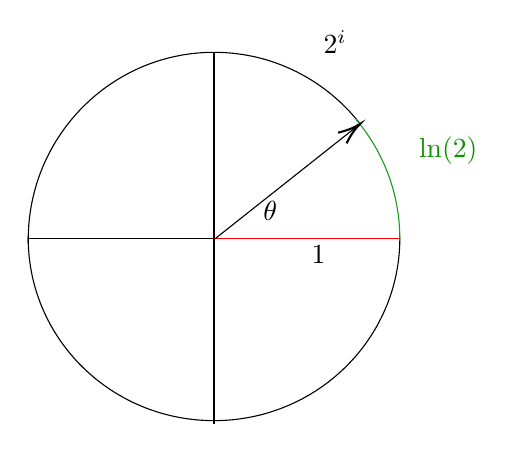
\begin{tikzpicture}[x=0.75pt,y=0.75pt,yscale=-1,xscale=1]
%uncomment if require: \path (0,300); %set diagram left start at 0, and has height of 300

%Straight Lines [id:da5300201460555855] 
\draw    (100,164.5) -- (189.5,164.5) ;
%Straight Lines [id:da7209499549539827] 
\draw    (189.5,254) -- (189.5,75) ;
%Shape: Arc [id:dp1477018513826992] 
\draw  [draw opacity=0] (100,167.2) .. controls (99.99,166.57) and (99.98,165.94) .. (99.98,165.31) .. controls (99.98,115.43) and (140.06,75) .. (189.51,75) .. controls (218.06,75) and (243.49,88.49) .. (259.88,109.49) -- (189.51,165.31) -- cycle ; \draw  [color={rgb, 255:red, 0; green, 0; blue, 0 }  ,draw opacity=1 ] (100,167.2) .. controls (99.99,166.57) and (99.98,165.94) .. (99.98,165.31) .. controls (99.98,115.43) and (140.06,75) .. (189.51,75) .. controls (218.06,75) and (243.49,88.49) .. (259.88,109.49) ;
%Straight Lines [id:da8647831039135583] 
\draw [color={rgb, 255:red, 255; green, 0; blue, 0 }  ,draw opacity=1 ]   (189.5,164.5) -- (279.02,164.5) ;
%Shape: Arc [id:dp5268217987140125] 
\draw  [draw opacity=0] (279.01,164.2) .. controls (279.01,164.3) and (279.02,164.4) .. (279.02,164.5) .. controls (279.02,213.08) and (238.94,252.46) .. (189.5,252.46) .. controls (140.06,252.46) and (99.98,213.08) .. (99.98,164.5) .. controls (99.98,164.29) and (99.99,164.08) .. (99.99,163.88) -- (189.5,164.5) -- cycle ; \draw   (279.01,164.2) .. controls (279.01,164.3) and (279.02,164.4) .. (279.02,164.5) .. controls (279.02,213.08) and (238.94,252.46) .. (189.5,252.46) .. controls (140.06,252.46) and (99.98,213.08) .. (99.98,164.5) .. controls (99.98,164.29) and (99.99,164.08) .. (99.99,163.88) ;
%Shape: Arc [id:dp1302089202448049] 
\draw  [draw opacity=0] (257.91,107.34) .. controls (271.09,122.89) and (279.03,143.02) .. (279.01,164.98) -- (189.91,164.9) -- cycle ; \draw  [color={rgb, 255:red, 22; green, 156; blue, 30 }  ,draw opacity=1 ] (257.91,107.34) .. controls (271.09,122.89) and (279.03,143.02) .. (279.01,164.98) ;
%Straight Lines [id:da04674799293912846] 
\draw    (189.91,164.9) -- (258.31,110.73) ;
\draw [shift={(259.88,109.49)}, rotate = 501.62] [color={rgb, 255:red, 0; green, 0; blue, 0 }  ][line width=0.75]    (10.93,-3.29) .. controls (6.95,-1.4) and (3.31,-0.3) .. (0,0) .. controls (3.31,0.3) and (6.95,1.4) .. (10.93,3.29)   ;

% Text Node
\draw (235.25,166.9) node [anchor=north west][inner sep=0.75pt]    {$1$};
% Text Node
\draw (287,114.4) node [anchor=north west][inner sep=0.75pt]  [color={rgb, 255:red, 12; green, 148; blue, 0 }  ,opacity=1 ]  {$\ln( 2)$};
% Text Node
\draw (241,63.4) node [anchor=north west][inner sep=0.75pt]    {$2^{i}$};
% Text Node
\draw (212,145.4) node [anchor=north west][inner sep=0.75pt]    {$\theta $};


\end{tikzpicture}

The rule \( (a^{b})^{c} = a^{bc} \) says that if we take \( p^c \)
but we express our base proportion \( p \)
as a exponentiation of a different proportion \( p = a^b \),
then the result can be expressed as \( a^{bc} \).

\begin{tikzpicture}[x=0.75pt,y=0.75pt,yscale=-1,xscale=1]
%uncomment if require: \path (0,300); %set diagram left start at 0, and has height of 300

%Curve Lines [id:da4423317108802115] 
\draw [color={rgb, 255:red, 255; green, 0; blue, 0 }  ,draw opacity=1 ]   (77.15,205.12) .. controls (201.44,203.62) and (289.8,139.23) .. (295.79,37.4) ;
%Straight Lines [id:da9534342452823479] 
\draw    (75.65,247.05) -- (297.28,247.05) ;
%Straight Lines [id:da33389606852560494] 
\draw    (75.65,35.9) -- (75.65,247.05) ;
%Shape: Circle [id:dp26393026690295507] 
\draw   (163,192) .. controls (163,190.9) and (163.9,190) .. (165,190) .. controls (166.1,190) and (167,190.9) .. (167,192) .. controls (167,193.1) and (166.1,194) .. (165,194) .. controls (163.9,194) and (163,193.1) .. (163,192) -- cycle ;
%Shape: Circle [id:dp10820914245059055] 
\draw   (123,201) .. controls (123,199.9) and (123.9,199) .. (125,199) .. controls (126.1,199) and (127,199.9) .. (127,201) .. controls (127,202.1) and (126.1,203) .. (125,203) .. controls (123.9,203) and (123,202.1) .. (123,201) -- cycle ;
%Shape: Circle [id:dp5803203757563192] 
\draw   (202,176) .. controls (202,174.9) and (202.9,174) .. (204,174) .. controls (205.1,174) and (206,174.9) .. (206,176) .. controls (206,177.1) and (205.1,178) .. (204,178) .. controls (202.9,178) and (202,177.1) .. (202,176) -- cycle ;
%Shape: Circle [id:dp5182181490141611] 
\draw   (255,137) .. controls (255,135.9) and (255.9,135) .. (257,135) .. controls (258.1,135) and (259,135.9) .. (259,137) .. controls (259,138.1) and (258.1,139) .. (257,139) .. controls (255.9,139) and (255,138.1) .. (255,137) -- cycle ;

% Text Node
\draw (71.9,262.4) node [anchor=north west][inner sep=0.75pt]    {$0$};
% Text Node
\draw (45,196.4) node [anchor=north west][inner sep=0.75pt]    {$1$};
% Text Node
\draw (167,193.4) node [anchor=north west][inner sep=0.75pt]  [color={rgb, 255:red, 255; green, 0; blue, 4 }  ,opacity=1 ]  {$e$};
% Text Node
\draw (163,263.4) node [anchor=north west][inner sep=0.75pt]    {$1$};
% Text Node
\draw (150,55.4) node [anchor=north west][inner sep=0.75pt]    {$e^{t}$};
% Text Node
\draw (127,202.4) node [anchor=north west][inner sep=0.75pt]    {$a$};
% Text Node
\draw (208,179.4) node [anchor=north west][inner sep=0.75pt]    {$b$};
% Text Node
\draw (261,140.4) node [anchor=north west][inner sep=0.75pt]    {$c$};


\end{tikzpicture}


The rule \( (ab)^c = a^c b^c \) says that if we take \( p^c \)
but we express our base proportion \( p \)
as a product of different proportions \( p = ab \),
then the result can be expressed as \( a^c b^{c} \).

\begin{tikzpicture}[x=0.75pt,y=0.75pt,yscale=-1,xscale=1]
%uncomment if require: \path (0,300); %set diagram left start at 0, and has height of 300

%Straight Lines [id:da34800919926202234] 
\draw [color={rgb, 255:red, 0; green, 0; blue, 0 }  ,draw opacity=1 ]   (99.75,227.18) -- (330.71,112.81) ;
\draw [shift={(332.5,111.93)}, rotate = 513.6600000000001] [color={rgb, 255:red, 0; green, 0; blue, 0 }  ,draw opacity=1 ][line width=0.75]    (10.93,-3.29) .. controls (6.95,-1.4) and (3.31,-0.3) .. (0,0) .. controls (3.31,0.3) and (6.95,1.4) .. (10.93,3.29)   ;
%Straight Lines [id:da63748929084913] 
\draw [color={rgb, 255:red, 255; green, 0; blue, 0 }  ,draw opacity=1 ]   (99.75,227.18) -- (219.09,168.63) ;
\draw [shift={(220.88,167.75)}, rotate = 513.87] [color={rgb, 255:red, 255; green, 0; blue, 0 }  ,draw opacity=1 ][line width=0.75]    (10.93,-3.29) .. controls (6.95,-1.4) and (3.31,-0.3) .. (0,0) .. controls (3.31,0.3) and (6.95,1.4) .. (10.93,3.29)   ;
%Straight Lines [id:da537720110515903] 
\draw [color={rgb, 255:red, 0; green, 95; blue, 255 }  ,draw opacity=1 ]   (220.88,167.75) -- (164.39,73.1) ;
\draw [shift={(163.36,71.38)}, rotate = 419.16999999999996] [color={rgb, 255:red, 0; green, 95; blue, 255 }  ,draw opacity=1 ][line width=0.75]    (10.93,-3.29) .. controls (6.95,-1.4) and (3.31,-0.3) .. (0,0) .. controls (3.31,0.3) and (6.95,1.4) .. (10.93,3.29)   ;
%Straight Lines [id:da16959396821644424] 
\draw    (99.75,227.18) -- (162.61,73.23) ;
\draw [shift={(163.36,71.38)}, rotate = 472.21] [color={rgb, 255:red, 0; green, 0; blue, 0 }  ][line width=0.75]    (10.93,-3.29) .. controls (6.95,-1.4) and (3.31,-0.3) .. (0,0) .. controls (3.31,0.3) and (6.95,1.4) .. (10.93,3.29)   ;
%Straight Lines [id:da8403058073952824] 
\draw    (99.75,227.18) -- (162.61,73.23) ;
\draw [shift={(163.36,71.38)}, rotate = 472.21] [color={rgb, 255:red, 0; green, 0; blue, 0 }  ][line width=0.75]    (10.93,-3.29) .. controls (6.95,-1.4) and (3.31,-0.3) .. (0,0) .. controls (3.31,0.3) and (6.95,1.4) .. (10.93,3.29)   ;

% Text Node
\draw (222.83,178.77) node [anchor=north west][inner sep=0.75pt]  [color={rgb, 255:red, 255; green, 0; blue, 0 }  ,opacity=1 ]  {$p=P_{u}( v)$};
% Text Node
\draw (202.31,100.35) node [anchor=north west][inner sep=0.75pt]  [color={rgb, 255:red, 0; green, 104; blue, 255 }  ,opacity=1 ]  {$v -p$};
% Text Node
\draw (149.98,43.4) node [anchor=north west][inner sep=0.75pt]    {$v$};
% Text Node
\draw (341.98,110.4) node [anchor=north west][inner sep=0.75pt]    {$u$};


\end{tikzpicture}



\subsubsection{Logarithm}

If exponentiation measure growth given time,
then the logarithm asks how much time is needed until we grow to a given amount.
Or even better, the amount of time needed to reach a certain proportion of growth.
Take \( b^t \) which measure continuous growth at a proportion of \( b \) per time step
starting at \( t = 0 \) with \( b^t = 1 \).
Then \( \log_b(c) \) is the amount of time needed to reach \( c \).
Thus, if \( \log_b(c) = t \), then \( b^t = c \).

\begin{tikzpicture}[x=0.75pt,y=0.75pt,yscale=-1,xscale=1]
%uncomment if require: \path (0,300); %set diagram left start at 0, and has height of 300

%Shape: Circle [id:dp6722596476060768] 
\draw   (103,86.25) .. controls (103,78.93) and (108.93,73) .. (116.25,73) .. controls (123.57,73) and (129.5,78.93) .. (129.5,86.25) .. controls (129.5,93.57) and (123.57,99.5) .. (116.25,99.5) .. controls (108.93,99.5) and (103,93.57) .. (103,86.25) -- cycle ;
%Shape: Circle [id:dp74444730195737] 
\draw   (140,86.25) .. controls (140,78.93) and (145.93,73) .. (153.25,73) .. controls (160.57,73) and (166.5,78.93) .. (166.5,86.25) .. controls (166.5,93.57) and (160.57,99.5) .. (153.25,99.5) .. controls (145.93,99.5) and (140,93.57) .. (140,86.25) -- cycle ;
%Shape: Circle [id:dp9832620880412448] 
\draw   (230,86.25) .. controls (230,78.93) and (235.93,73) .. (243.25,73) .. controls (250.57,73) and (256.5,78.93) .. (256.5,86.25) .. controls (256.5,93.57) and (250.57,99.5) .. (243.25,99.5) .. controls (235.93,99.5) and (230,93.57) .. (230,86.25) -- cycle ;
%Shape: Brace [id:dp5022040197364186] 
\draw   (236.5,57) .. controls (236.5,52.33) and (234.17,50) .. (229.5,50) -- (188,50) .. controls (181.33,50) and (178,47.67) .. (178,43) .. controls (178,47.67) and (174.67,50) .. (168,50)(171,50) -- (126.5,50) .. controls (121.83,50) and (119.5,52.33) .. (119.5,57) ;
%Shape: Square [id:dp23486906391618334] 
\draw   (100,171) -- (126.5,171) -- (126.5,197.5) -- (100,197.5) -- cycle ;
%Shape: Square [id:dp8514361205022334] 
\draw   (134,171) -- (160.5,171) -- (160.5,197.5) -- (134,197.5) -- cycle ;
%Shape: Square [id:dp5165693986546934] 
\draw   (226,172) -- (252.5,172) -- (252.5,198.5) -- (226,198.5) -- cycle ;
%Shape: Brace [id:dp2319346457546657] 
\draw   (110.5,221) .. controls (110.5,225.67) and (112.83,228) .. (117.5,228) -- (169,228) .. controls (175.67,228) and (179,230.33) .. (179,235) .. controls (179,230.33) and (182.33,228) .. (189,228)(186,228) -- (240.5,228) .. controls (245.17,228) and (247.5,225.67) .. (247.5,221) ;
%Straight Lines [id:da9665534418589774] 
\draw    (113.25,170) -- (113.25,131) ;
\draw [shift={(113.25,129)}, rotate = 450] [color={rgb, 255:red, 0; green, 0; blue, 0 }  ][line width=0.75]    (10.93,-3.29) .. controls (6.95,-1.4) and (3.31,-0.3) .. (0,0) .. controls (3.31,0.3) and (6.95,1.4) .. (10.93,3.29)   ;
%Straight Lines [id:da2232187544111287] 
\draw    (148.25,171) -- (148.25,132) ;
\draw [shift={(148.25,130)}, rotate = 450] [color={rgb, 255:red, 0; green, 0; blue, 0 }  ][line width=0.75]    (10.93,-3.29) .. controls (6.95,-1.4) and (3.31,-0.3) .. (0,0) .. controls (3.31,0.3) and (6.95,1.4) .. (10.93,3.29)   ;
%Straight Lines [id:da8929455340252761] 
\draw    (240.25,169) -- (240.25,130) ;
\draw [shift={(240.25,128)}, rotate = 450] [color={rgb, 255:red, 0; green, 0; blue, 0 }  ][line width=0.75]    (10.93,-3.29) .. controls (6.95,-1.4) and (3.31,-0.3) .. (0,0) .. controls (3.31,0.3) and (6.95,1.4) .. (10.93,3.29)   ;

% Text Node
\draw (185,86.4) node [anchor=north west][inner sep=0.75pt]    {$\dotsc $};
% Text Node
\draw (170,14.4) node [anchor=north west][inner sep=0.75pt]    {$n$};
% Text Node
\draw (180,187.4) node [anchor=north west][inner sep=0.75pt]    {$\dotsc $};
% Text Node
\draw (175,248.4) node [anchor=north west][inner sep=0.75pt]    {$r$};


\end{tikzpicture}



By this definition, we have \( b^{\log_b(c)} = c \).

For \( \log_b(ac) \),
we can interpret this as the amount of time until we reach a factor of \( ac \).


\tikzset{every picture/.style={line width=0.75pt}} %set default line width to 0.75pt        

\begin{tikzpicture}[x=0.75pt,y=0.75pt,yscale=-1,xscale=1]
%uncomment if require: \path (0,300); %set diagram left start at 0, and has height of 300

%Shape: Axis 2D [id:dp7522167816409159] 
\draw  (50,242) -- (419.5,242)(97.5,8) -- (97.5,267) (412.5,237) -- (419.5,242) -- (412.5,247) (92.5,15) -- (97.5,8) -- (102.5,15) (146.5,237) -- (146.5,247)(195.5,237) -- (195.5,247)(244.5,237) -- (244.5,247)(293.5,237) -- (293.5,247)(342.5,237) -- (342.5,247)(391.5,237) -- (391.5,247)(92.5,193) -- (102.5,193)(92.5,144) -- (102.5,144)(92.5,95) -- (102.5,95)(92.5,46) -- (102.5,46) ;
\draw   ;
%Shape: Circle [id:dp1800333897763694] 
\draw   (297,120.75) .. controls (297,117.57) and (299.57,115) .. (302.75,115) .. controls (305.93,115) and (308.5,117.57) .. (308.5,120.75) .. controls (308.5,123.93) and (305.93,126.5) .. (302.75,126.5) .. controls (299.57,126.5) and (297,123.93) .. (297,120.75) -- cycle ;
%Curve Lines [id:da6744184215507455] 
\draw    (98,171) .. controls (107.79,163.66) and (111.03,107.89) .. (139.27,154.95) .. controls (167.5,202) and (206.02,160.39) .. (242.5,187) .. controls (278.98,213.61) and (267.5,117) .. (297,120.75) ;
%Straight Lines [id:da042236632067626734] 
\draw [color={rgb, 255:red, 255; green, 0; blue, 0 }  ,draw opacity=1 ]   (302,103) -- (302,62) ;
\draw [shift={(302,60)}, rotate = 450] [color={rgb, 255:red, 255; green, 0; blue, 0 }  ,draw opacity=1 ][line width=0.75]    (10.93,-3.29) .. controls (6.95,-1.4) and (3.31,-0.3) .. (0,0) .. controls (3.31,0.3) and (6.95,1.4) .. (10.93,3.29)   ;
%Straight Lines [id:da8879089279998805] 
\draw [color={rgb, 255:red, 255; green, 0; blue, 0 }  ,draw opacity=1 ]   (301.75,136.5) -- (301.75,175) ;
\draw [shift={(301.75,177)}, rotate = 270] [color={rgb, 255:red, 255; green, 0; blue, 0 }  ,draw opacity=1 ][line width=0.75]    (10.93,-3.29) .. controls (6.95,-1.4) and (3.31,-0.3) .. (0,0) .. controls (3.31,0.3) and (6.95,1.4) .. (10.93,3.29)   ;
%Straight Lines [id:da984234265425485] 
\draw  [dash pattern={on 0.84pt off 2.51pt}]  (302.75,126.5) -- (302.75,245) ;
%Straight Lines [id:da851126430686476] 
\draw [color={rgb, 255:red, 0; green, 42; blue, 255 }  ,draw opacity=1 ]   (267,260) -- (298.5,260) ;
\draw [shift={(300.5,260)}, rotate = 180] [color={rgb, 255:red, 0; green, 42; blue, 255 }  ,draw opacity=1 ][line width=0.75]    (10.93,-3.29) .. controls (6.95,-1.4) and (3.31,-0.3) .. (0,0) .. controls (3.31,0.3) and (6.95,1.4) .. (10.93,3.29)   ;


\end{tikzpicture}


But since \( ac \) is just \( a \) multiplied by a proportion of \( c \),
we can just find the times for \( b \) and \( c \) separately:
\[ \log_b(ac) = \log_b(a) + \log_b(c). \]

Now for \( log_b(a^c) \),
we want to know the time until we reach a proportion \( a^c \).
We can just figure out the time until \( a \),
then just repeat the time as needed
\[ \log_b(a^c) = c \cdot \log_b(a). \]

\tikzset{every picture/.style={line width=0.75pt}} %set default line width to 0.75pt        

\tikzset{every picture/.style={line width=0.75pt}} %set default line width to 0.75pt        

\noindent
\begin{tikzpicture}[x=0.75pt,y=0.75pt,yscale=-1,xscale=1]
%uncomment if require: \path (0,300); %set diagram left start at 0, and has height of 300

%Shape: Axis 2D [id:dp049849838656989] 
\draw  (70,180) -- (535.5,180)(183.5,60) -- (183.5,282) (528.5,175) -- (535.5,180) -- (528.5,185) (178.5,67) -- (183.5,60) -- (188.5,67) (216.5,175) -- (216.5,185)(249.5,175) -- (249.5,185)(282.5,175) -- (282.5,185)(315.5,175) -- (315.5,185)(348.5,175) -- (348.5,185)(381.5,175) -- (381.5,185)(414.5,175) -- (414.5,185)(447.5,175) -- (447.5,185)(480.5,175) -- (480.5,185)(513.5,175) -- (513.5,185)(150.5,175) -- (150.5,185)(117.5,175) -- (117.5,185)(84.5,175) -- (84.5,185)(178.5,147) -- (188.5,147)(178.5,114) -- (188.5,114)(178.5,81) -- (188.5,81)(178.5,213) -- (188.5,213)(178.5,246) -- (188.5,246) ;
\draw   ;
%Straight Lines [id:da9974234043672462] 
\draw    (183.5,180) -- (276.05,92.38) ;
\draw [shift={(277.5,91)}, rotate = 496.57] [color={rgb, 255:red, 0; green, 0; blue, 0 }  ][line width=0.75]    (10.93,-3.29) .. controls (6.95,-1.4) and (3.31,-0.3) .. (0,0) .. controls (3.31,0.3) and (6.95,1.4) .. (10.93,3.29)   ;
%Straight Lines [id:da20657379122009134] 
\draw    (183.5,180) -- (273.67,219.2) ;
\draw [shift={(275.5,220)}, rotate = 203.5] [color={rgb, 255:red, 0; green, 0; blue, 0 }  ][line width=0.75]    (10.93,-3.29) .. controls (6.95,-1.4) and (3.31,-0.3) .. (0,0) .. controls (3.31,0.3) and (6.95,1.4) .. (10.93,3.29)   ;
%Shape: Arc [id:dp5803037905068104] 
\draw  [draw opacity=0] (200.9,165.06) .. controls (203.44,166.14) and (205.18,168.69) .. (205.1,171.61) .. controls (205.01,174.63) and (202.98,177.14) .. (200.25,177.99) -- (198.21,171.4) -- cycle ; \draw   (200.9,165.06) .. controls (203.44,166.14) and (205.18,168.69) .. (205.1,171.61) .. controls (205.01,174.63) and (202.98,177.14) .. (200.25,177.99) ;
%Shape: Arc [id:dp7047653051043884] 
\draw  [draw opacity=0] (207.18,181.49) .. controls (209,182.26) and (210.25,184.09) .. (210.19,186.18) .. controls (210.12,188.34) and (208.68,190.13) .. (206.72,190.74) -- (205.26,186.03) -- cycle ; \draw   (207.18,181.49) .. controls (209,182.26) and (210.25,184.09) .. (210.19,186.18) .. controls (210.12,188.34) and (208.68,190.13) .. (206.72,190.74) ;
%Straight Lines [id:da4324446373354387] 
\draw [color={rgb, 255:red, 255; green, 0; blue, 0 }  ,draw opacity=1 ]   (183.5,180) -- (513.56,97.49) ;
\draw [shift={(515.5,97)}, rotate = 525.96] [color={rgb, 255:red, 255; green, 0; blue, 0 }  ,draw opacity=1 ][line width=0.75]    (10.93,-3.29) .. controls (6.95,-1.4) and (3.31,-0.3) .. (0,0) .. controls (3.31,0.3) and (6.95,1.4) .. (10.93,3.29)   ;
%Shape: Arc [id:dp5325215380673752] 
\draw  [draw opacity=0] (235.18,168.49) .. controls (237,169.26) and (238.25,171.09) .. (238.19,173.18) .. controls (238.12,175.34) and (236.68,177.13) .. (234.72,177.74) -- (233.26,173.03) -- cycle ; \draw  [color={rgb, 255:red, 255; green, 0; blue, 0 }  ,draw opacity=1 ] (235.18,168.49) .. controls (237,169.26) and (238.25,171.09) .. (238.19,173.18) .. controls (238.12,175.34) and (236.68,177.13) .. (234.72,177.74) ;

% Text Node
\draw (250,72.4) node [anchor=north west][inner sep=0.75pt]    {$z_{1}$};
% Text Node
\draw (274,228.4) node [anchor=north west][inner sep=0.75pt]    {$z_{2}$};
% Text Node
\draw (208,154.4) node [anchor=north west][inner sep=0.75pt]  [font=\footnotesize]  {$\theta $};
% Text Node
\draw (221,180.4) node [anchor=north west][inner sep=0.75pt]  [font=\footnotesize]  {$\phi $};
% Text Node
\draw (211,125.4) node [anchor=north west][inner sep=0.75pt]    {$r$};
% Text Node
\draw (221,208.4) node [anchor=north west][inner sep=0.75pt]    {$p$};
% Text Node
\draw (370,105.4) node [anchor=north west][inner sep=0.75pt]  [color={rgb, 255:red, 255; green, 0; blue, 0 }  ,opacity=1 ]  {$rp$};
% Text Node
\draw (525,84.4) node [anchor=north west][inner sep=0.75pt]  [color={rgb, 255:red, 255; green, 0; blue, 0 }  ,opacity=1 ]  {$z_{1} z_{2}$};
% Text Node
\draw (265,161.4) node [anchor=north west][inner sep=0.75pt]  [font=\footnotesize,color={rgb, 255:red, 255; green, 0; blue, 0 }  ,opacity=1 ]  {$\theta +\phi $};


\end{tikzpicture}

\newpage
We know we can convert between different proportions.

\noindent
\begin{tikzpicture}[x=0.75pt,y=0.75pt,yscale=-0.8,xscale=0.8]
%uncomment if require: \path (0,300); %set diagram left start at 0, and has height of 300

%Curve Lines [id:da16505242416400712] 
\draw [color={rgb, 255:red, 255; green, 0; blue, 0 }  ,draw opacity=1 ]   (103.15,205.12) .. controls (227.44,203.62) and (315.8,139.23) .. (321.79,37.4) ;
%Straight Lines [id:da7267676985584549] 
\draw    (101.65,247.05) -- (323.28,247.05) ;
%Straight Lines [id:da4645289606705647] 
\draw    (101.65,35.9) -- (101.65,247.05) ;
%Shape: Circle [id:dp39770385046406675] 
\draw   (189,192) .. controls (189,190.9) and (189.9,190) .. (191,190) .. controls (192.1,190) and (193,190.9) .. (193,192) .. controls (193,193.1) and (192.1,194) .. (191,194) .. controls (189.9,194) and (189,193.1) .. (189,192) -- cycle ;
%Straight Lines [id:da1118098783506678] 
\draw [color={rgb, 255:red, 0; green, 50; blue, 255 }  ,draw opacity=1 ]   (103.15,205.12) -- (256.5,160) ;
%Shape: Brace [id:dp33401170253306967] 
\draw   (102,208) .. controls (102,212.67) and (104.33,215) .. (109,215) -- (172.25,215) .. controls (178.92,215) and (182.25,217.33) .. (182.25,222) .. controls (182.25,217.33) and (185.58,215) .. (192.25,215)(189.25,215) -- (255.5,215) .. controls (260.17,215) and (262.5,212.67) .. (262.5,208) ;
%Curve Lines [id:da702343555310466] 
\draw [color={rgb, 255:red, 255; green, 0; blue, 0 }  ,draw opacity=1 ]   (408.15,203.12) .. controls (532.44,201.62) and (620.8,137.23) .. (626.79,35.4) ;
%Straight Lines [id:da5457712288003155] 
\draw    (406.65,245.05) -- (628.28,245.05) ;
%Straight Lines [id:da6145389316373155] 
\draw    (406.65,33.9) -- (406.65,245.05) ;
%Shape: Circle [id:dp8592795818420744] 
\draw   (494,190) .. controls (494,188.9) and (494.9,188) .. (496,188) .. controls (497.1,188) and (498,188.9) .. (498,190) .. controls (498,191.1) and (497.1,192) .. (496,192) .. controls (494.9,192) and (494,191.1) .. (494,190) -- cycle ;
%Straight Lines [id:da9754483079369636] 
\draw [color={rgb, 255:red, 0; green, 42; blue, 255 }  ,draw opacity=1 ]   (461.5,198) -- (619.5,76) ;
%Shape: Brace [id:dp4810786659509392] 
\draw   (463,205) .. controls (463,209.67) and (465.33,212) .. (470,212) -- (533.25,212) .. controls (539.92,212) and (543.25,214.33) .. (543.25,219) .. controls (543.25,214.33) and (546.58,212) .. (553.25,212)(550.25,212) -- (616.5,212) .. controls (621.17,212) and (623.5,209.67) .. (623.5,205) ;

% Text Node
\draw (97.9,262.4) node [anchor=north west][inner sep=0.75pt]    {$0$};
% Text Node
\draw (71,196.4) node [anchor=north west][inner sep=0.75pt]    {$1$};
% Text Node
\draw (193,193.4) node [anchor=north west][inner sep=0.75pt]    {$b$};
% Text Node
\draw (189,263.4) node [anchor=north west][inner sep=0.75pt]    {$1$};
% Text Node
\draw (178,155.4) node [anchor=north west][inner sep=0.75pt]  [color={rgb, 255:red, 0; green, 33; blue, 255 }  ,opacity=1 ]  {$b^{c}$};
% Text Node
\draw (177,222.4) node [anchor=north west][inner sep=0.75pt]    {$c$};
% Text Node
\draw (402.9,260.4) node [anchor=north west][inner sep=0.75pt]    {$0$};
% Text Node
\draw (376,194.4) node [anchor=north west][inner sep=0.75pt]    {$1$};
% Text Node
\draw (498,191.4) node [anchor=north west][inner sep=0.75pt]    {$b$};
% Text Node
\draw (494,261.4) node [anchor=north west][inner sep=0.75pt]    {$1$};
% Text Node
\draw (518,120.4) node [anchor=north west][inner sep=0.75pt]  [color={rgb, 255:red, 0; green, 24; blue, 255 }  ,opacity=1 ]  {$b^{c}$};
% Text Node
\draw (538,219.4) node [anchor=north west][inner sep=0.75pt]    {$c$};
% Text Node
\draw (258.5,163.4) node [anchor=north west][inner sep=0.75pt]    {$b^{c}$};
% Text Node
\draw (450,176.4) node [anchor=north west][inner sep=0.75pt]    {$a$};
% Text Node
\draw (621.5,79.4) node [anchor=north west][inner sep=0.75pt]    {$ab^{c}$};

\end{tikzpicture}

Suppose we have \( b^t \) but we want to talk about it in terms of \( a \).
We know the amount of time it takes to reach amount \( b \) at a growth ratio of \( a \)
is \( p = \log_a(b) \).
So \( b^t = a^{pt} \).


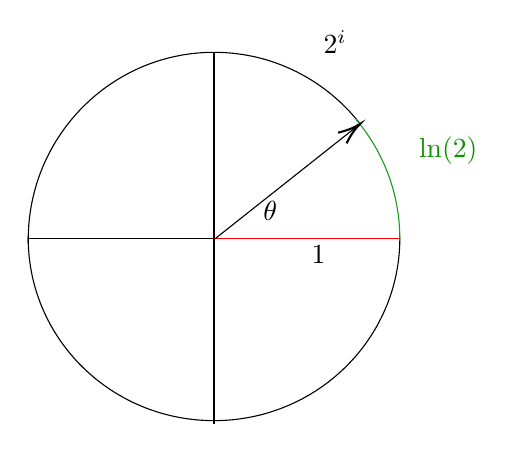
\begin{tikzpicture}[x=0.75pt,y=0.75pt,yscale=-1,xscale=1]
%uncomment if require: \path (0,300); %set diagram left start at 0, and has height of 300

%Straight Lines [id:da5300201460555855] 
\draw    (100,164.5) -- (189.5,164.5) ;
%Straight Lines [id:da7209499549539827] 
\draw    (189.5,254) -- (189.5,75) ;
%Shape: Arc [id:dp1477018513826992] 
\draw  [draw opacity=0] (100,167.2) .. controls (99.99,166.57) and (99.98,165.94) .. (99.98,165.31) .. controls (99.98,115.43) and (140.06,75) .. (189.51,75) .. controls (218.06,75) and (243.49,88.49) .. (259.88,109.49) -- (189.51,165.31) -- cycle ; \draw  [color={rgb, 255:red, 0; green, 0; blue, 0 }  ,draw opacity=1 ] (100,167.2) .. controls (99.99,166.57) and (99.98,165.94) .. (99.98,165.31) .. controls (99.98,115.43) and (140.06,75) .. (189.51,75) .. controls (218.06,75) and (243.49,88.49) .. (259.88,109.49) ;
%Straight Lines [id:da8647831039135583] 
\draw [color={rgb, 255:red, 255; green, 0; blue, 0 }  ,draw opacity=1 ]   (189.5,164.5) -- (279.02,164.5) ;
%Shape: Arc [id:dp5268217987140125] 
\draw  [draw opacity=0] (279.01,164.2) .. controls (279.01,164.3) and (279.02,164.4) .. (279.02,164.5) .. controls (279.02,213.08) and (238.94,252.46) .. (189.5,252.46) .. controls (140.06,252.46) and (99.98,213.08) .. (99.98,164.5) .. controls (99.98,164.29) and (99.99,164.08) .. (99.99,163.88) -- (189.5,164.5) -- cycle ; \draw   (279.01,164.2) .. controls (279.01,164.3) and (279.02,164.4) .. (279.02,164.5) .. controls (279.02,213.08) and (238.94,252.46) .. (189.5,252.46) .. controls (140.06,252.46) and (99.98,213.08) .. (99.98,164.5) .. controls (99.98,164.29) and (99.99,164.08) .. (99.99,163.88) ;
%Shape: Arc [id:dp1302089202448049] 
\draw  [draw opacity=0] (257.91,107.34) .. controls (271.09,122.89) and (279.03,143.02) .. (279.01,164.98) -- (189.91,164.9) -- cycle ; \draw  [color={rgb, 255:red, 22; green, 156; blue, 30 }  ,draw opacity=1 ] (257.91,107.34) .. controls (271.09,122.89) and (279.03,143.02) .. (279.01,164.98) ;
%Straight Lines [id:da04674799293912846] 
\draw    (189.91,164.9) -- (258.31,110.73) ;
\draw [shift={(259.88,109.49)}, rotate = 501.62] [color={rgb, 255:red, 0; green, 0; blue, 0 }  ][line width=0.75]    (10.93,-3.29) .. controls (6.95,-1.4) and (3.31,-0.3) .. (0,0) .. controls (3.31,0.3) and (6.95,1.4) .. (10.93,3.29)   ;

% Text Node
\draw (235.25,166.9) node [anchor=north west][inner sep=0.75pt]    {$1$};
% Text Node
\draw (287,114.4) node [anchor=north west][inner sep=0.75pt]  [color={rgb, 255:red, 12; green, 148; blue, 0 }  ,opacity=1 ]  {$\ln( 2)$};
% Text Node
\draw (241,63.4) node [anchor=north west][inner sep=0.75pt]    {$2^{i}$};
% Text Node
\draw (212,145.4) node [anchor=north west][inner sep=0.75pt]    {$\theta $};


\end{tikzpicture}

And \( \log_a(b^t) = t \cdot \log_a(b) \), and \( t = \frac{\log_a(b^t)}{\log_a(b)} \).


\begin{tikzpicture}[x=0.75pt,y=0.75pt,yscale=-1,xscale=1]
%uncomment if require: \path (0,300); %set diagram left start at 0, and has height of 300

%Curve Lines [id:da4423317108802115] 
\draw [color={rgb, 255:red, 255; green, 0; blue, 0 }  ,draw opacity=1 ]   (77.15,205.12) .. controls (201.44,203.62) and (289.8,139.23) .. (295.79,37.4) ;
%Straight Lines [id:da9534342452823479] 
\draw    (75.65,247.05) -- (297.28,247.05) ;
%Straight Lines [id:da33389606852560494] 
\draw    (75.65,35.9) -- (75.65,247.05) ;
%Shape: Circle [id:dp26393026690295507] 
\draw   (163,192) .. controls (163,190.9) and (163.9,190) .. (165,190) .. controls (166.1,190) and (167,190.9) .. (167,192) .. controls (167,193.1) and (166.1,194) .. (165,194) .. controls (163.9,194) and (163,193.1) .. (163,192) -- cycle ;
%Shape: Circle [id:dp10820914245059055] 
\draw   (123,201) .. controls (123,199.9) and (123.9,199) .. (125,199) .. controls (126.1,199) and (127,199.9) .. (127,201) .. controls (127,202.1) and (126.1,203) .. (125,203) .. controls (123.9,203) and (123,202.1) .. (123,201) -- cycle ;
%Shape: Circle [id:dp5803203757563192] 
\draw   (202,176) .. controls (202,174.9) and (202.9,174) .. (204,174) .. controls (205.1,174) and (206,174.9) .. (206,176) .. controls (206,177.1) and (205.1,178) .. (204,178) .. controls (202.9,178) and (202,177.1) .. (202,176) -- cycle ;
%Shape: Circle [id:dp5182181490141611] 
\draw   (255,137) .. controls (255,135.9) and (255.9,135) .. (257,135) .. controls (258.1,135) and (259,135.9) .. (259,137) .. controls (259,138.1) and (258.1,139) .. (257,139) .. controls (255.9,139) and (255,138.1) .. (255,137) -- cycle ;

% Text Node
\draw (71.9,262.4) node [anchor=north west][inner sep=0.75pt]    {$0$};
% Text Node
\draw (45,196.4) node [anchor=north west][inner sep=0.75pt]    {$1$};
% Text Node
\draw (167,193.4) node [anchor=north west][inner sep=0.75pt]  [color={rgb, 255:red, 255; green, 0; blue, 4 }  ,opacity=1 ]  {$e$};
% Text Node
\draw (163,263.4) node [anchor=north west][inner sep=0.75pt]    {$1$};
% Text Node
\draw (150,55.4) node [anchor=north west][inner sep=0.75pt]    {$e^{t}$};
% Text Node
\draw (127,202.4) node [anchor=north west][inner sep=0.75pt]    {$a$};
% Text Node
\draw (208,179.4) node [anchor=north west][inner sep=0.75pt]    {$b$};
% Text Node
\draw (261,140.4) node [anchor=north west][inner sep=0.75pt]    {$c$};


\end{tikzpicture}

So \( \log \) is just a measurement, but in terms of the length of 1
which is just the length until we reach a proportion of the base.
Since all exponential functions are really the same,
we can just think of them all in terms of a common base, say \( e \).
Then our measuring stick of 1 is just \( \ln(e) = 1\).

So if we are given \( \log_a(x) \), this just means
the length until we reach a multiple of \( x \),
but measured if 1 was the length until \( a \).
Thus \( \log_a(x) = \frac{\ln(x)}{\ln(a)} \).


\subsection{Distribution, Linearity}

Multiplication is related to linearity.
It distributes over addition \( a(b + c) = ab + ac \).
It preserves the proportions between \( b \) and \( c \).
Note that this is \( b/c \) and division is the inverse of multiplication.
It takes 0 to 0 which is the additive identity.

Likewise, exponentiation distributes over multiplication
\( (ab)^x = a^x b^x \).
It preserves logarithms \( \log_a(b) = \log_{a^x}(b^x) \).
It takes 0 to 1 which is the multiplicative identity.

Both linear functions and exponential functions are memoryless and self-similar.


\newpage
\section{Functions}

\subsection{Linear Functions}

A linear function \( f(x) = cx \) is a constant scaling.
It has the properties that it maps 0 to 0,
that it preserves addition: \( f(a+b) = f(a) + f(b) \),
and that it preserves additional scaling: \( f(cx) = cf(x) \).
This results in something like the real line being mapped to an evenly spaced out line.
The scaling constant \( c \) is the slope.

\begin{tikzpicture}[x=0.75pt,y=0.75pt,yscale=-1,xscale=1]
%uncomment if require: \path (0,300); %set diagram left start at 0, and has height of 300

%Shape: Circle [id:dp6722596476060768] 
\draw   (103,86.25) .. controls (103,78.93) and (108.93,73) .. (116.25,73) .. controls (123.57,73) and (129.5,78.93) .. (129.5,86.25) .. controls (129.5,93.57) and (123.57,99.5) .. (116.25,99.5) .. controls (108.93,99.5) and (103,93.57) .. (103,86.25) -- cycle ;
%Shape: Circle [id:dp74444730195737] 
\draw   (140,86.25) .. controls (140,78.93) and (145.93,73) .. (153.25,73) .. controls (160.57,73) and (166.5,78.93) .. (166.5,86.25) .. controls (166.5,93.57) and (160.57,99.5) .. (153.25,99.5) .. controls (145.93,99.5) and (140,93.57) .. (140,86.25) -- cycle ;
%Shape: Circle [id:dp9832620880412448] 
\draw   (230,86.25) .. controls (230,78.93) and (235.93,73) .. (243.25,73) .. controls (250.57,73) and (256.5,78.93) .. (256.5,86.25) .. controls (256.5,93.57) and (250.57,99.5) .. (243.25,99.5) .. controls (235.93,99.5) and (230,93.57) .. (230,86.25) -- cycle ;
%Shape: Brace [id:dp5022040197364186] 
\draw   (236.5,57) .. controls (236.5,52.33) and (234.17,50) .. (229.5,50) -- (188,50) .. controls (181.33,50) and (178,47.67) .. (178,43) .. controls (178,47.67) and (174.67,50) .. (168,50)(171,50) -- (126.5,50) .. controls (121.83,50) and (119.5,52.33) .. (119.5,57) ;
%Shape: Square [id:dp23486906391618334] 
\draw   (100,171) -- (126.5,171) -- (126.5,197.5) -- (100,197.5) -- cycle ;
%Shape: Square [id:dp8514361205022334] 
\draw   (134,171) -- (160.5,171) -- (160.5,197.5) -- (134,197.5) -- cycle ;
%Shape: Square [id:dp5165693986546934] 
\draw   (226,172) -- (252.5,172) -- (252.5,198.5) -- (226,198.5) -- cycle ;
%Shape: Brace [id:dp2319346457546657] 
\draw   (110.5,221) .. controls (110.5,225.67) and (112.83,228) .. (117.5,228) -- (169,228) .. controls (175.67,228) and (179,230.33) .. (179,235) .. controls (179,230.33) and (182.33,228) .. (189,228)(186,228) -- (240.5,228) .. controls (245.17,228) and (247.5,225.67) .. (247.5,221) ;
%Straight Lines [id:da9665534418589774] 
\draw    (113.25,170) -- (113.25,131) ;
\draw [shift={(113.25,129)}, rotate = 450] [color={rgb, 255:red, 0; green, 0; blue, 0 }  ][line width=0.75]    (10.93,-3.29) .. controls (6.95,-1.4) and (3.31,-0.3) .. (0,0) .. controls (3.31,0.3) and (6.95,1.4) .. (10.93,3.29)   ;
%Straight Lines [id:da2232187544111287] 
\draw    (148.25,171) -- (148.25,132) ;
\draw [shift={(148.25,130)}, rotate = 450] [color={rgb, 255:red, 0; green, 0; blue, 0 }  ][line width=0.75]    (10.93,-3.29) .. controls (6.95,-1.4) and (3.31,-0.3) .. (0,0) .. controls (3.31,0.3) and (6.95,1.4) .. (10.93,3.29)   ;
%Straight Lines [id:da8929455340252761] 
\draw    (240.25,169) -- (240.25,130) ;
\draw [shift={(240.25,128)}, rotate = 450] [color={rgb, 255:red, 0; green, 0; blue, 0 }  ][line width=0.75]    (10.93,-3.29) .. controls (6.95,-1.4) and (3.31,-0.3) .. (0,0) .. controls (3.31,0.3) and (6.95,1.4) .. (10.93,3.29)   ;

% Text Node
\draw (185,86.4) node [anchor=north west][inner sep=0.75pt]    {$\dotsc $};
% Text Node
\draw (170,14.4) node [anchor=north west][inner sep=0.75pt]    {$n$};
% Text Node
\draw (180,187.4) node [anchor=north west][inner sep=0.75pt]    {$\dotsc $};
% Text Node
\draw (175,248.4) node [anchor=north west][inner sep=0.75pt]    {$r$};


\end{tikzpicture}


Translations of linear functions are called affine functions.

\subsection{Composition}

Think of \( f(2x) \) as running through the function twice as fast.
Think of \( f(x + 2) \) as starting running through the function at 2.
Given some \( g(x) \), we can think of \( f(g(x)) \)
where the rate we are running through \( f \) is determined by \( g(x) \).

We know we can combine the operations of addition, multiplication, powers, etc.
to make new functions.
We can consider these operations themselves functions.
For example, take
\[ f(x) = 3x^2 + (x - 1)^4 - 2^x. \]
We can rewrite this as
\[ f(x) = 3f_1(x) + f_2(f_3(x)) - f_1(x) \]
where the operations are each replaced with their abstraction in the form of a function.

\subsection{Graphs}

A real function is a single dimensional measurement of quantity.
With one variable, the quantity is parameterized in one dimension by the input.
In other words, as we vary the input dimension, what do we get in the output dimension?
We can graph this relationship as such.

\tikzset{every picture/.style={line width=0.75pt}} %set default line width to 0.75pt        

\tikzset{every picture/.style={line width=0.75pt}} %set default line width to 0.75pt        

\begin{tikzpicture}[x=0.75pt,y=0.75pt,yscale=-1,xscale=1]
%uncomment if require: \path (0,300); %set diagram left start at 0, and has height of 300

%Shape: Axis 2D [id:dp7522167816409159] 
\draw  (50,242) -- (419.5,242)(97.5,8) -- (97.5,267) (412.5,237) -- (419.5,242) -- (412.5,247) (92.5,15) -- (97.5,8) -- (102.5,15) (146.5,237) -- (146.5,247)(195.5,237) -- (195.5,247)(244.5,237) -- (244.5,247)(293.5,237) -- (293.5,247)(342.5,237) -- (342.5,247)(391.5,237) -- (391.5,247)(92.5,193) -- (102.5,193)(92.5,144) -- (102.5,144)(92.5,95) -- (102.5,95)(92.5,46) -- (102.5,46) ;
\draw   ;
%Shape: Circle [id:dp1800333897763694] 
\draw   (297,120.75) .. controls (297,117.57) and (299.57,115) .. (302.75,115) .. controls (305.93,115) and (308.5,117.57) .. (308.5,120.75) .. controls (308.5,123.93) and (305.93,126.5) .. (302.75,126.5) .. controls (299.57,126.5) and (297,123.93) .. (297,120.75) -- cycle ;
%Curve Lines [id:da6744184215507455] 
\draw    (98,171) .. controls (107.79,163.66) and (111.03,107.89) .. (139.27,154.95) .. controls (167.5,202) and (206.02,160.39) .. (242.5,187) .. controls (278.98,213.61) and (267.5,117) .. (297,120.75) ;
%Straight Lines [id:da042236632067626734] 
\draw [color={rgb, 255:red, 255; green, 0; blue, 0 }  ,draw opacity=1 ]   (302,103) -- (302,62) ;
\draw [shift={(302,60)}, rotate = 450] [color={rgb, 255:red, 255; green, 0; blue, 0 }  ,draw opacity=1 ][line width=0.75]    (10.93,-3.29) .. controls (6.95,-1.4) and (3.31,-0.3) .. (0,0) .. controls (3.31,0.3) and (6.95,1.4) .. (10.93,3.29)   ;
%Straight Lines [id:da8879089279998805] 
\draw [color={rgb, 255:red, 255; green, 0; blue, 0 }  ,draw opacity=1 ]   (301.75,136.5) -- (301.75,175) ;
\draw [shift={(301.75,177)}, rotate = 270] [color={rgb, 255:red, 255; green, 0; blue, 0 }  ,draw opacity=1 ][line width=0.75]    (10.93,-3.29) .. controls (6.95,-1.4) and (3.31,-0.3) .. (0,0) .. controls (3.31,0.3) and (6.95,1.4) .. (10.93,3.29)   ;
%Straight Lines [id:da984234265425485] 
\draw  [dash pattern={on 0.84pt off 2.51pt}]  (302.75,126.5) -- (302.75,245) ;
%Straight Lines [id:da851126430686476] 
\draw [color={rgb, 255:red, 0; green, 42; blue, 255 }  ,draw opacity=1 ]   (267,260) -- (298.5,260) ;
\draw [shift={(300.5,260)}, rotate = 180] [color={rgb, 255:red, 0; green, 42; blue, 255 }  ,draw opacity=1 ][line width=0.75]    (10.93,-3.29) .. controls (6.95,-1.4) and (3.31,-0.3) .. (0,0) .. controls (3.31,0.3) and (6.95,1.4) .. (10.93,3.29)   ;


\end{tikzpicture}


We don't care about the location of the "ball", we only care about the height.


\subsection{Inverse}

For an invertible \( f \), we have \( f\inv \).
Imagine turning the graph of \( f \) counterclockwise.

\tikzset{every picture/.style={line width=0.75pt}} %set default line width to 0.75pt        

\noindent
\begin{tikzpicture}[x=0.75pt,y=0.75pt,yscale=-1,xscale=1]
%uncomment if require: \path (0,300); %set diagram left start at 0, and has height of 300

%Shape: Axis 2D [id:dp049849838656989] 
\draw  (70,180) -- (535.5,180)(183.5,60) -- (183.5,282) (528.5,175) -- (535.5,180) -- (528.5,185) (178.5,67) -- (183.5,60) -- (188.5,67) (216.5,175) -- (216.5,185)(249.5,175) -- (249.5,185)(282.5,175) -- (282.5,185)(315.5,175) -- (315.5,185)(348.5,175) -- (348.5,185)(381.5,175) -- (381.5,185)(414.5,175) -- (414.5,185)(447.5,175) -- (447.5,185)(480.5,175) -- (480.5,185)(513.5,175) -- (513.5,185)(150.5,175) -- (150.5,185)(117.5,175) -- (117.5,185)(84.5,175) -- (84.5,185)(178.5,147) -- (188.5,147)(178.5,114) -- (188.5,114)(178.5,81) -- (188.5,81)(178.5,213) -- (188.5,213)(178.5,246) -- (188.5,246) ;
\draw   ;
%Straight Lines [id:da9974234043672462] 
\draw    (183.5,180) -- (276.05,92.38) ;
\draw [shift={(277.5,91)}, rotate = 496.57] [color={rgb, 255:red, 0; green, 0; blue, 0 }  ][line width=0.75]    (10.93,-3.29) .. controls (6.95,-1.4) and (3.31,-0.3) .. (0,0) .. controls (3.31,0.3) and (6.95,1.4) .. (10.93,3.29)   ;
%Straight Lines [id:da20657379122009134] 
\draw    (183.5,180) -- (273.67,219.2) ;
\draw [shift={(275.5,220)}, rotate = 203.5] [color={rgb, 255:red, 0; green, 0; blue, 0 }  ][line width=0.75]    (10.93,-3.29) .. controls (6.95,-1.4) and (3.31,-0.3) .. (0,0) .. controls (3.31,0.3) and (6.95,1.4) .. (10.93,3.29)   ;
%Shape: Arc [id:dp5803037905068104] 
\draw  [draw opacity=0] (200.9,165.06) .. controls (203.44,166.14) and (205.18,168.69) .. (205.1,171.61) .. controls (205.01,174.63) and (202.98,177.14) .. (200.25,177.99) -- (198.21,171.4) -- cycle ; \draw   (200.9,165.06) .. controls (203.44,166.14) and (205.18,168.69) .. (205.1,171.61) .. controls (205.01,174.63) and (202.98,177.14) .. (200.25,177.99) ;
%Shape: Arc [id:dp7047653051043884] 
\draw  [draw opacity=0] (207.18,181.49) .. controls (209,182.26) and (210.25,184.09) .. (210.19,186.18) .. controls (210.12,188.34) and (208.68,190.13) .. (206.72,190.74) -- (205.26,186.03) -- cycle ; \draw   (207.18,181.49) .. controls (209,182.26) and (210.25,184.09) .. (210.19,186.18) .. controls (210.12,188.34) and (208.68,190.13) .. (206.72,190.74) ;
%Straight Lines [id:da4324446373354387] 
\draw [color={rgb, 255:red, 255; green, 0; blue, 0 }  ,draw opacity=1 ]   (183.5,180) -- (513.56,97.49) ;
\draw [shift={(515.5,97)}, rotate = 525.96] [color={rgb, 255:red, 255; green, 0; blue, 0 }  ,draw opacity=1 ][line width=0.75]    (10.93,-3.29) .. controls (6.95,-1.4) and (3.31,-0.3) .. (0,0) .. controls (3.31,0.3) and (6.95,1.4) .. (10.93,3.29)   ;
%Shape: Arc [id:dp5325215380673752] 
\draw  [draw opacity=0] (235.18,168.49) .. controls (237,169.26) and (238.25,171.09) .. (238.19,173.18) .. controls (238.12,175.34) and (236.68,177.13) .. (234.72,177.74) -- (233.26,173.03) -- cycle ; \draw  [color={rgb, 255:red, 255; green, 0; blue, 0 }  ,draw opacity=1 ] (235.18,168.49) .. controls (237,169.26) and (238.25,171.09) .. (238.19,173.18) .. controls (238.12,175.34) and (236.68,177.13) .. (234.72,177.74) ;

% Text Node
\draw (250,72.4) node [anchor=north west][inner sep=0.75pt]    {$z_{1}$};
% Text Node
\draw (274,228.4) node [anchor=north west][inner sep=0.75pt]    {$z_{2}$};
% Text Node
\draw (208,154.4) node [anchor=north west][inner sep=0.75pt]  [font=\footnotesize]  {$\theta $};
% Text Node
\draw (221,180.4) node [anchor=north west][inner sep=0.75pt]  [font=\footnotesize]  {$\phi $};
% Text Node
\draw (211,125.4) node [anchor=north west][inner sep=0.75pt]    {$r$};
% Text Node
\draw (221,208.4) node [anchor=north west][inner sep=0.75pt]    {$p$};
% Text Node
\draw (370,105.4) node [anchor=north west][inner sep=0.75pt]  [color={rgb, 255:red, 255; green, 0; blue, 0 }  ,opacity=1 ]  {$rp$};
% Text Node
\draw (525,84.4) node [anchor=north west][inner sep=0.75pt]  [color={rgb, 255:red, 255; green, 0; blue, 0 }  ,opacity=1 ]  {$z_{1} z_{2}$};
% Text Node
\draw (265,161.4) node [anchor=north west][inner sep=0.75pt]  [font=\footnotesize,color={rgb, 255:red, 255; green, 0; blue, 0 }  ,opacity=1 ]  {$\theta +\phi $};


\end{tikzpicture}

Then the inverse function is what we get if we try to stretch the vertical axis
in order to get a straight line.

\noindent
\begin{tikzpicture}[x=0.75pt,y=0.75pt,yscale=-0.8,xscale=0.8]
%uncomment if require: \path (0,300); %set diagram left start at 0, and has height of 300

%Curve Lines [id:da16505242416400712] 
\draw [color={rgb, 255:red, 255; green, 0; blue, 0 }  ,draw opacity=1 ]   (103.15,205.12) .. controls (227.44,203.62) and (315.8,139.23) .. (321.79,37.4) ;
%Straight Lines [id:da7267676985584549] 
\draw    (101.65,247.05) -- (323.28,247.05) ;
%Straight Lines [id:da4645289606705647] 
\draw    (101.65,35.9) -- (101.65,247.05) ;
%Shape: Circle [id:dp39770385046406675] 
\draw   (189,192) .. controls (189,190.9) and (189.9,190) .. (191,190) .. controls (192.1,190) and (193,190.9) .. (193,192) .. controls (193,193.1) and (192.1,194) .. (191,194) .. controls (189.9,194) and (189,193.1) .. (189,192) -- cycle ;
%Straight Lines [id:da1118098783506678] 
\draw [color={rgb, 255:red, 0; green, 50; blue, 255 }  ,draw opacity=1 ]   (103.15,205.12) -- (256.5,160) ;
%Shape: Brace [id:dp33401170253306967] 
\draw   (102,208) .. controls (102,212.67) and (104.33,215) .. (109,215) -- (172.25,215) .. controls (178.92,215) and (182.25,217.33) .. (182.25,222) .. controls (182.25,217.33) and (185.58,215) .. (192.25,215)(189.25,215) -- (255.5,215) .. controls (260.17,215) and (262.5,212.67) .. (262.5,208) ;
%Curve Lines [id:da702343555310466] 
\draw [color={rgb, 255:red, 255; green, 0; blue, 0 }  ,draw opacity=1 ]   (408.15,203.12) .. controls (532.44,201.62) and (620.8,137.23) .. (626.79,35.4) ;
%Straight Lines [id:da5457712288003155] 
\draw    (406.65,245.05) -- (628.28,245.05) ;
%Straight Lines [id:da6145389316373155] 
\draw    (406.65,33.9) -- (406.65,245.05) ;
%Shape: Circle [id:dp8592795818420744] 
\draw   (494,190) .. controls (494,188.9) and (494.9,188) .. (496,188) .. controls (497.1,188) and (498,188.9) .. (498,190) .. controls (498,191.1) and (497.1,192) .. (496,192) .. controls (494.9,192) and (494,191.1) .. (494,190) -- cycle ;
%Straight Lines [id:da9754483079369636] 
\draw [color={rgb, 255:red, 0; green, 42; blue, 255 }  ,draw opacity=1 ]   (461.5,198) -- (619.5,76) ;
%Shape: Brace [id:dp4810786659509392] 
\draw   (463,205) .. controls (463,209.67) and (465.33,212) .. (470,212) -- (533.25,212) .. controls (539.92,212) and (543.25,214.33) .. (543.25,219) .. controls (543.25,214.33) and (546.58,212) .. (553.25,212)(550.25,212) -- (616.5,212) .. controls (621.17,212) and (623.5,209.67) .. (623.5,205) ;

% Text Node
\draw (97.9,262.4) node [anchor=north west][inner sep=0.75pt]    {$0$};
% Text Node
\draw (71,196.4) node [anchor=north west][inner sep=0.75pt]    {$1$};
% Text Node
\draw (193,193.4) node [anchor=north west][inner sep=0.75pt]    {$b$};
% Text Node
\draw (189,263.4) node [anchor=north west][inner sep=0.75pt]    {$1$};
% Text Node
\draw (178,155.4) node [anchor=north west][inner sep=0.75pt]  [color={rgb, 255:red, 0; green, 33; blue, 255 }  ,opacity=1 ]  {$b^{c}$};
% Text Node
\draw (177,222.4) node [anchor=north west][inner sep=0.75pt]    {$c$};
% Text Node
\draw (402.9,260.4) node [anchor=north west][inner sep=0.75pt]    {$0$};
% Text Node
\draw (376,194.4) node [anchor=north west][inner sep=0.75pt]    {$1$};
% Text Node
\draw (498,191.4) node [anchor=north west][inner sep=0.75pt]    {$b$};
% Text Node
\draw (494,261.4) node [anchor=north west][inner sep=0.75pt]    {$1$};
% Text Node
\draw (518,120.4) node [anchor=north west][inner sep=0.75pt]  [color={rgb, 255:red, 0; green, 24; blue, 255 }  ,opacity=1 ]  {$b^{c}$};
% Text Node
\draw (538,219.4) node [anchor=north west][inner sep=0.75pt]    {$c$};
% Text Node
\draw (258.5,163.4) node [anchor=north west][inner sep=0.75pt]    {$b^{c}$};
% Text Node
\draw (450,176.4) node [anchor=north west][inner sep=0.75pt]    {$a$};
% Text Node
\draw (621.5,79.4) node [anchor=north west][inner sep=0.75pt]    {$ab^{c}$};

\end{tikzpicture}

\newpage
\section{Trig Functions}

\subsection{Circles}

Take a circle with radius \( r \).
We define \( \pi \) to be the ratio of half the circumference to the radius.
In other words, the half arc is \( \pi \) times as long as the radius.
     

\begin{tikzpicture}[x=0.75pt,y=0.75pt,yscale=-1,xscale=1]
%uncomment if require: \path (0,300); %set diagram left start at 0, and has height of 300

%Shape: Circle [id:dp6722596476060768] 
\draw   (103,86.25) .. controls (103,78.93) and (108.93,73) .. (116.25,73) .. controls (123.57,73) and (129.5,78.93) .. (129.5,86.25) .. controls (129.5,93.57) and (123.57,99.5) .. (116.25,99.5) .. controls (108.93,99.5) and (103,93.57) .. (103,86.25) -- cycle ;
%Shape: Circle [id:dp74444730195737] 
\draw   (140,86.25) .. controls (140,78.93) and (145.93,73) .. (153.25,73) .. controls (160.57,73) and (166.5,78.93) .. (166.5,86.25) .. controls (166.5,93.57) and (160.57,99.5) .. (153.25,99.5) .. controls (145.93,99.5) and (140,93.57) .. (140,86.25) -- cycle ;
%Shape: Circle [id:dp9832620880412448] 
\draw   (230,86.25) .. controls (230,78.93) and (235.93,73) .. (243.25,73) .. controls (250.57,73) and (256.5,78.93) .. (256.5,86.25) .. controls (256.5,93.57) and (250.57,99.5) .. (243.25,99.5) .. controls (235.93,99.5) and (230,93.57) .. (230,86.25) -- cycle ;
%Shape: Brace [id:dp5022040197364186] 
\draw   (236.5,57) .. controls (236.5,52.33) and (234.17,50) .. (229.5,50) -- (188,50) .. controls (181.33,50) and (178,47.67) .. (178,43) .. controls (178,47.67) and (174.67,50) .. (168,50)(171,50) -- (126.5,50) .. controls (121.83,50) and (119.5,52.33) .. (119.5,57) ;
%Shape: Square [id:dp23486906391618334] 
\draw   (100,171) -- (126.5,171) -- (126.5,197.5) -- (100,197.5) -- cycle ;
%Shape: Square [id:dp8514361205022334] 
\draw   (134,171) -- (160.5,171) -- (160.5,197.5) -- (134,197.5) -- cycle ;
%Shape: Square [id:dp5165693986546934] 
\draw   (226,172) -- (252.5,172) -- (252.5,198.5) -- (226,198.5) -- cycle ;
%Shape: Brace [id:dp2319346457546657] 
\draw   (110.5,221) .. controls (110.5,225.67) and (112.83,228) .. (117.5,228) -- (169,228) .. controls (175.67,228) and (179,230.33) .. (179,235) .. controls (179,230.33) and (182.33,228) .. (189,228)(186,228) -- (240.5,228) .. controls (245.17,228) and (247.5,225.67) .. (247.5,221) ;
%Straight Lines [id:da9665534418589774] 
\draw    (113.25,170) -- (113.25,131) ;
\draw [shift={(113.25,129)}, rotate = 450] [color={rgb, 255:red, 0; green, 0; blue, 0 }  ][line width=0.75]    (10.93,-3.29) .. controls (6.95,-1.4) and (3.31,-0.3) .. (0,0) .. controls (3.31,0.3) and (6.95,1.4) .. (10.93,3.29)   ;
%Straight Lines [id:da2232187544111287] 
\draw    (148.25,171) -- (148.25,132) ;
\draw [shift={(148.25,130)}, rotate = 450] [color={rgb, 255:red, 0; green, 0; blue, 0 }  ][line width=0.75]    (10.93,-3.29) .. controls (6.95,-1.4) and (3.31,-0.3) .. (0,0) .. controls (3.31,0.3) and (6.95,1.4) .. (10.93,3.29)   ;
%Straight Lines [id:da8929455340252761] 
\draw    (240.25,169) -- (240.25,130) ;
\draw [shift={(240.25,128)}, rotate = 450] [color={rgb, 255:red, 0; green, 0; blue, 0 }  ][line width=0.75]    (10.93,-3.29) .. controls (6.95,-1.4) and (3.31,-0.3) .. (0,0) .. controls (3.31,0.3) and (6.95,1.4) .. (10.93,3.29)   ;

% Text Node
\draw (185,86.4) node [anchor=north west][inner sep=0.75pt]    {$\dotsc $};
% Text Node
\draw (170,14.4) node [anchor=north west][inner sep=0.75pt]    {$n$};
% Text Node
\draw (180,187.4) node [anchor=north west][inner sep=0.75pt]    {$\dotsc $};
% Text Node
\draw (175,248.4) node [anchor=north west][inner sep=0.75pt]    {$r$};


\end{tikzpicture}


Then the whole circumference is \( 2\pi r \).

\subsubsection{Radians}

Radians are a measure of angle by considering ratios of arc lengths to the radius.
Start with the rightmost point on the circle.
If we consider the point on the circle a certain angle away counterclockwise,
what is the ratio of the covered arc length to the radius?
How much do we have to multiply the radius by to reach the same length?

Thus an angle of \( \pi \) radians is half the angle around a circle,
and an angle of \( \pi/4 \) is an eighth of the angle.

\tikzset{every picture/.style={line width=0.75pt}} %set default line width to 0.75pt        

\tikzset{every picture/.style={line width=0.75pt}} %set default line width to 0.75pt        

\begin{tikzpicture}[x=0.75pt,y=0.75pt,yscale=-1,xscale=1]
%uncomment if require: \path (0,300); %set diagram left start at 0, and has height of 300

%Shape: Axis 2D [id:dp7522167816409159] 
\draw  (50,242) -- (419.5,242)(97.5,8) -- (97.5,267) (412.5,237) -- (419.5,242) -- (412.5,247) (92.5,15) -- (97.5,8) -- (102.5,15) (146.5,237) -- (146.5,247)(195.5,237) -- (195.5,247)(244.5,237) -- (244.5,247)(293.5,237) -- (293.5,247)(342.5,237) -- (342.5,247)(391.5,237) -- (391.5,247)(92.5,193) -- (102.5,193)(92.5,144) -- (102.5,144)(92.5,95) -- (102.5,95)(92.5,46) -- (102.5,46) ;
\draw   ;
%Shape: Circle [id:dp1800333897763694] 
\draw   (297,120.75) .. controls (297,117.57) and (299.57,115) .. (302.75,115) .. controls (305.93,115) and (308.5,117.57) .. (308.5,120.75) .. controls (308.5,123.93) and (305.93,126.5) .. (302.75,126.5) .. controls (299.57,126.5) and (297,123.93) .. (297,120.75) -- cycle ;
%Curve Lines [id:da6744184215507455] 
\draw    (98,171) .. controls (107.79,163.66) and (111.03,107.89) .. (139.27,154.95) .. controls (167.5,202) and (206.02,160.39) .. (242.5,187) .. controls (278.98,213.61) and (267.5,117) .. (297,120.75) ;
%Straight Lines [id:da042236632067626734] 
\draw [color={rgb, 255:red, 255; green, 0; blue, 0 }  ,draw opacity=1 ]   (302,103) -- (302,62) ;
\draw [shift={(302,60)}, rotate = 450] [color={rgb, 255:red, 255; green, 0; blue, 0 }  ,draw opacity=1 ][line width=0.75]    (10.93,-3.29) .. controls (6.95,-1.4) and (3.31,-0.3) .. (0,0) .. controls (3.31,0.3) and (6.95,1.4) .. (10.93,3.29)   ;
%Straight Lines [id:da8879089279998805] 
\draw [color={rgb, 255:red, 255; green, 0; blue, 0 }  ,draw opacity=1 ]   (301.75,136.5) -- (301.75,175) ;
\draw [shift={(301.75,177)}, rotate = 270] [color={rgb, 255:red, 255; green, 0; blue, 0 }  ,draw opacity=1 ][line width=0.75]    (10.93,-3.29) .. controls (6.95,-1.4) and (3.31,-0.3) .. (0,0) .. controls (3.31,0.3) and (6.95,1.4) .. (10.93,3.29)   ;
%Straight Lines [id:da984234265425485] 
\draw  [dash pattern={on 0.84pt off 2.51pt}]  (302.75,126.5) -- (302.75,245) ;
%Straight Lines [id:da851126430686476] 
\draw [color={rgb, 255:red, 0; green, 42; blue, 255 }  ,draw opacity=1 ]   (267,260) -- (298.5,260) ;
\draw [shift={(300.5,260)}, rotate = 180] [color={rgb, 255:red, 0; green, 42; blue, 255 }  ,draw opacity=1 ][line width=0.75]    (10.93,-3.29) .. controls (6.95,-1.4) and (3.31,-0.3) .. (0,0) .. controls (3.31,0.3) and (6.95,1.4) .. (10.93,3.29)   ;


\end{tikzpicture}

Note that an angle of 0 and an angle of \( 2\pi \) is the same.
Thus, angles in radians are an equivalence class, or the reals quotient \( 2\pi \).

Because we are working with ratios,
it is convenient to just visualize a unit circle with a radius of 1.

\subsection{Sine, Cosine, and Tangent}

Given a circle, the maximum height and the maximum width is the radius \( r \).
The functions \( \sin \) and \( \cos \),
given an angle in radians,
tells us how much of this maximum height and width is covered by the point at the angle.

\tikzset{every picture/.style={line width=0.75pt}} %set default line width to 0.75pt        

\tikzset{every picture/.style={line width=0.75pt}} %set default line width to 0.75pt        

\noindent
\begin{tikzpicture}[x=0.75pt,y=0.75pt,yscale=-1,xscale=1]
%uncomment if require: \path (0,300); %set diagram left start at 0, and has height of 300

%Shape: Axis 2D [id:dp049849838656989] 
\draw  (70,180) -- (535.5,180)(183.5,60) -- (183.5,282) (528.5,175) -- (535.5,180) -- (528.5,185) (178.5,67) -- (183.5,60) -- (188.5,67) (216.5,175) -- (216.5,185)(249.5,175) -- (249.5,185)(282.5,175) -- (282.5,185)(315.5,175) -- (315.5,185)(348.5,175) -- (348.5,185)(381.5,175) -- (381.5,185)(414.5,175) -- (414.5,185)(447.5,175) -- (447.5,185)(480.5,175) -- (480.5,185)(513.5,175) -- (513.5,185)(150.5,175) -- (150.5,185)(117.5,175) -- (117.5,185)(84.5,175) -- (84.5,185)(178.5,147) -- (188.5,147)(178.5,114) -- (188.5,114)(178.5,81) -- (188.5,81)(178.5,213) -- (188.5,213)(178.5,246) -- (188.5,246) ;
\draw   ;
%Straight Lines [id:da9974234043672462] 
\draw    (183.5,180) -- (276.05,92.38) ;
\draw [shift={(277.5,91)}, rotate = 496.57] [color={rgb, 255:red, 0; green, 0; blue, 0 }  ][line width=0.75]    (10.93,-3.29) .. controls (6.95,-1.4) and (3.31,-0.3) .. (0,0) .. controls (3.31,0.3) and (6.95,1.4) .. (10.93,3.29)   ;
%Straight Lines [id:da20657379122009134] 
\draw    (183.5,180) -- (273.67,219.2) ;
\draw [shift={(275.5,220)}, rotate = 203.5] [color={rgb, 255:red, 0; green, 0; blue, 0 }  ][line width=0.75]    (10.93,-3.29) .. controls (6.95,-1.4) and (3.31,-0.3) .. (0,0) .. controls (3.31,0.3) and (6.95,1.4) .. (10.93,3.29)   ;
%Shape: Arc [id:dp5803037905068104] 
\draw  [draw opacity=0] (200.9,165.06) .. controls (203.44,166.14) and (205.18,168.69) .. (205.1,171.61) .. controls (205.01,174.63) and (202.98,177.14) .. (200.25,177.99) -- (198.21,171.4) -- cycle ; \draw   (200.9,165.06) .. controls (203.44,166.14) and (205.18,168.69) .. (205.1,171.61) .. controls (205.01,174.63) and (202.98,177.14) .. (200.25,177.99) ;
%Shape: Arc [id:dp7047653051043884] 
\draw  [draw opacity=0] (207.18,181.49) .. controls (209,182.26) and (210.25,184.09) .. (210.19,186.18) .. controls (210.12,188.34) and (208.68,190.13) .. (206.72,190.74) -- (205.26,186.03) -- cycle ; \draw   (207.18,181.49) .. controls (209,182.26) and (210.25,184.09) .. (210.19,186.18) .. controls (210.12,188.34) and (208.68,190.13) .. (206.72,190.74) ;
%Straight Lines [id:da4324446373354387] 
\draw [color={rgb, 255:red, 255; green, 0; blue, 0 }  ,draw opacity=1 ]   (183.5,180) -- (513.56,97.49) ;
\draw [shift={(515.5,97)}, rotate = 525.96] [color={rgb, 255:red, 255; green, 0; blue, 0 }  ,draw opacity=1 ][line width=0.75]    (10.93,-3.29) .. controls (6.95,-1.4) and (3.31,-0.3) .. (0,0) .. controls (3.31,0.3) and (6.95,1.4) .. (10.93,3.29)   ;
%Shape: Arc [id:dp5325215380673752] 
\draw  [draw opacity=0] (235.18,168.49) .. controls (237,169.26) and (238.25,171.09) .. (238.19,173.18) .. controls (238.12,175.34) and (236.68,177.13) .. (234.72,177.74) -- (233.26,173.03) -- cycle ; \draw  [color={rgb, 255:red, 255; green, 0; blue, 0 }  ,draw opacity=1 ] (235.18,168.49) .. controls (237,169.26) and (238.25,171.09) .. (238.19,173.18) .. controls (238.12,175.34) and (236.68,177.13) .. (234.72,177.74) ;

% Text Node
\draw (250,72.4) node [anchor=north west][inner sep=0.75pt]    {$z_{1}$};
% Text Node
\draw (274,228.4) node [anchor=north west][inner sep=0.75pt]    {$z_{2}$};
% Text Node
\draw (208,154.4) node [anchor=north west][inner sep=0.75pt]  [font=\footnotesize]  {$\theta $};
% Text Node
\draw (221,180.4) node [anchor=north west][inner sep=0.75pt]  [font=\footnotesize]  {$\phi $};
% Text Node
\draw (211,125.4) node [anchor=north west][inner sep=0.75pt]    {$r$};
% Text Node
\draw (221,208.4) node [anchor=north west][inner sep=0.75pt]    {$p$};
% Text Node
\draw (370,105.4) node [anchor=north west][inner sep=0.75pt]  [color={rgb, 255:red, 255; green, 0; blue, 0 }  ,opacity=1 ]  {$rp$};
% Text Node
\draw (525,84.4) node [anchor=north west][inner sep=0.75pt]  [color={rgb, 255:red, 255; green, 0; blue, 0 }  ,opacity=1 ]  {$z_{1} z_{2}$};
% Text Node
\draw (265,161.4) node [anchor=north west][inner sep=0.75pt]  [font=\footnotesize,color={rgb, 255:red, 255; green, 0; blue, 0 }  ,opacity=1 ]  {$\theta +\phi $};


\end{tikzpicture}

They give us the answer as a ratio of or as a percentage of \( r \).

Because the domain of these functions is a partition of the reals,
they are periodic with a period of \( 2\pi \).
This means
\[ \cos(x) = \cos(x + 2\pi) \]
and
\[ \sin(x) = \sin(x + 2\pi). \]

We can specify the coordinates of a point in two ways.
First, we can specify it's position along each axis (rectangular form):
\[ (r \cos(x), r \sin(x)), \]
or we can just give the radius and angle (polar form):
\[ (r, x). \]

\newpage
The function \( \tan \) is just the ratio

\tikzset{every picture/.style={line width=0.75pt}} %set default line width to 0.75pt        

\noindent
\begin{tikzpicture}[x=0.75pt,y=0.75pt,yscale=-0.8,xscale=0.8]
%uncomment if require: \path (0,300); %set diagram left start at 0, and has height of 300

%Curve Lines [id:da16505242416400712] 
\draw [color={rgb, 255:red, 255; green, 0; blue, 0 }  ,draw opacity=1 ]   (103.15,205.12) .. controls (227.44,203.62) and (315.8,139.23) .. (321.79,37.4) ;
%Straight Lines [id:da7267676985584549] 
\draw    (101.65,247.05) -- (323.28,247.05) ;
%Straight Lines [id:da4645289606705647] 
\draw    (101.65,35.9) -- (101.65,247.05) ;
%Shape: Circle [id:dp39770385046406675] 
\draw   (189,192) .. controls (189,190.9) and (189.9,190) .. (191,190) .. controls (192.1,190) and (193,190.9) .. (193,192) .. controls (193,193.1) and (192.1,194) .. (191,194) .. controls (189.9,194) and (189,193.1) .. (189,192) -- cycle ;
%Straight Lines [id:da1118098783506678] 
\draw [color={rgb, 255:red, 0; green, 50; blue, 255 }  ,draw opacity=1 ]   (103.15,205.12) -- (256.5,160) ;
%Shape: Brace [id:dp33401170253306967] 
\draw   (102,208) .. controls (102,212.67) and (104.33,215) .. (109,215) -- (172.25,215) .. controls (178.92,215) and (182.25,217.33) .. (182.25,222) .. controls (182.25,217.33) and (185.58,215) .. (192.25,215)(189.25,215) -- (255.5,215) .. controls (260.17,215) and (262.5,212.67) .. (262.5,208) ;
%Curve Lines [id:da702343555310466] 
\draw [color={rgb, 255:red, 255; green, 0; blue, 0 }  ,draw opacity=1 ]   (408.15,203.12) .. controls (532.44,201.62) and (620.8,137.23) .. (626.79,35.4) ;
%Straight Lines [id:da5457712288003155] 
\draw    (406.65,245.05) -- (628.28,245.05) ;
%Straight Lines [id:da6145389316373155] 
\draw    (406.65,33.9) -- (406.65,245.05) ;
%Shape: Circle [id:dp8592795818420744] 
\draw   (494,190) .. controls (494,188.9) and (494.9,188) .. (496,188) .. controls (497.1,188) and (498,188.9) .. (498,190) .. controls (498,191.1) and (497.1,192) .. (496,192) .. controls (494.9,192) and (494,191.1) .. (494,190) -- cycle ;
%Straight Lines [id:da9754483079369636] 
\draw [color={rgb, 255:red, 0; green, 42; blue, 255 }  ,draw opacity=1 ]   (461.5,198) -- (619.5,76) ;
%Shape: Brace [id:dp4810786659509392] 
\draw   (463,205) .. controls (463,209.67) and (465.33,212) .. (470,212) -- (533.25,212) .. controls (539.92,212) and (543.25,214.33) .. (543.25,219) .. controls (543.25,214.33) and (546.58,212) .. (553.25,212)(550.25,212) -- (616.5,212) .. controls (621.17,212) and (623.5,209.67) .. (623.5,205) ;

% Text Node
\draw (97.9,262.4) node [anchor=north west][inner sep=0.75pt]    {$0$};
% Text Node
\draw (71,196.4) node [anchor=north west][inner sep=0.75pt]    {$1$};
% Text Node
\draw (193,193.4) node [anchor=north west][inner sep=0.75pt]    {$b$};
% Text Node
\draw (189,263.4) node [anchor=north west][inner sep=0.75pt]    {$1$};
% Text Node
\draw (178,155.4) node [anchor=north west][inner sep=0.75pt]  [color={rgb, 255:red, 0; green, 33; blue, 255 }  ,opacity=1 ]  {$b^{c}$};
% Text Node
\draw (177,222.4) node [anchor=north west][inner sep=0.75pt]    {$c$};
% Text Node
\draw (402.9,260.4) node [anchor=north west][inner sep=0.75pt]    {$0$};
% Text Node
\draw (376,194.4) node [anchor=north west][inner sep=0.75pt]    {$1$};
% Text Node
\draw (498,191.4) node [anchor=north west][inner sep=0.75pt]    {$b$};
% Text Node
\draw (494,261.4) node [anchor=north west][inner sep=0.75pt]    {$1$};
% Text Node
\draw (518,120.4) node [anchor=north west][inner sep=0.75pt]  [color={rgb, 255:red, 0; green, 24; blue, 255 }  ,opacity=1 ]  {$b^{c}$};
% Text Node
\draw (538,219.4) node [anchor=north west][inner sep=0.75pt]    {$c$};
% Text Node
\draw (258.5,163.4) node [anchor=north west][inner sep=0.75pt]    {$b^{c}$};
% Text Node
\draw (450,176.4) node [anchor=north west][inner sep=0.75pt]    {$a$};
% Text Node
\draw (621.5,79.4) node [anchor=north west][inner sep=0.75pt]    {$ab^{c}$};

\end{tikzpicture}

We can think of this as the slope of the line through the point at the angle.


\newpage
\section{Complex Numbers}

The complex numbers are a number system or a field just like the reals.
Each complex number is made of two parts: the real part and the imaginary part.
We can represent these on a plane with one axis being real and the other being imaginary.
Take a complex number \( z = a + bi \).
    

\begin{tikzpicture}[x=0.75pt,y=0.75pt,yscale=-1,xscale=1]
%uncomment if require: \path (0,300); %set diagram left start at 0, and has height of 300

%Shape: Circle [id:dp6722596476060768] 
\draw   (103,86.25) .. controls (103,78.93) and (108.93,73) .. (116.25,73) .. controls (123.57,73) and (129.5,78.93) .. (129.5,86.25) .. controls (129.5,93.57) and (123.57,99.5) .. (116.25,99.5) .. controls (108.93,99.5) and (103,93.57) .. (103,86.25) -- cycle ;
%Shape: Circle [id:dp74444730195737] 
\draw   (140,86.25) .. controls (140,78.93) and (145.93,73) .. (153.25,73) .. controls (160.57,73) and (166.5,78.93) .. (166.5,86.25) .. controls (166.5,93.57) and (160.57,99.5) .. (153.25,99.5) .. controls (145.93,99.5) and (140,93.57) .. (140,86.25) -- cycle ;
%Shape: Circle [id:dp9832620880412448] 
\draw   (230,86.25) .. controls (230,78.93) and (235.93,73) .. (243.25,73) .. controls (250.57,73) and (256.5,78.93) .. (256.5,86.25) .. controls (256.5,93.57) and (250.57,99.5) .. (243.25,99.5) .. controls (235.93,99.5) and (230,93.57) .. (230,86.25) -- cycle ;
%Shape: Brace [id:dp5022040197364186] 
\draw   (236.5,57) .. controls (236.5,52.33) and (234.17,50) .. (229.5,50) -- (188,50) .. controls (181.33,50) and (178,47.67) .. (178,43) .. controls (178,47.67) and (174.67,50) .. (168,50)(171,50) -- (126.5,50) .. controls (121.83,50) and (119.5,52.33) .. (119.5,57) ;
%Shape: Square [id:dp23486906391618334] 
\draw   (100,171) -- (126.5,171) -- (126.5,197.5) -- (100,197.5) -- cycle ;
%Shape: Square [id:dp8514361205022334] 
\draw   (134,171) -- (160.5,171) -- (160.5,197.5) -- (134,197.5) -- cycle ;
%Shape: Square [id:dp5165693986546934] 
\draw   (226,172) -- (252.5,172) -- (252.5,198.5) -- (226,198.5) -- cycle ;
%Shape: Brace [id:dp2319346457546657] 
\draw   (110.5,221) .. controls (110.5,225.67) and (112.83,228) .. (117.5,228) -- (169,228) .. controls (175.67,228) and (179,230.33) .. (179,235) .. controls (179,230.33) and (182.33,228) .. (189,228)(186,228) -- (240.5,228) .. controls (245.17,228) and (247.5,225.67) .. (247.5,221) ;
%Straight Lines [id:da9665534418589774] 
\draw    (113.25,170) -- (113.25,131) ;
\draw [shift={(113.25,129)}, rotate = 450] [color={rgb, 255:red, 0; green, 0; blue, 0 }  ][line width=0.75]    (10.93,-3.29) .. controls (6.95,-1.4) and (3.31,-0.3) .. (0,0) .. controls (3.31,0.3) and (6.95,1.4) .. (10.93,3.29)   ;
%Straight Lines [id:da2232187544111287] 
\draw    (148.25,171) -- (148.25,132) ;
\draw [shift={(148.25,130)}, rotate = 450] [color={rgb, 255:red, 0; green, 0; blue, 0 }  ][line width=0.75]    (10.93,-3.29) .. controls (6.95,-1.4) and (3.31,-0.3) .. (0,0) .. controls (3.31,0.3) and (6.95,1.4) .. (10.93,3.29)   ;
%Straight Lines [id:da8929455340252761] 
\draw    (240.25,169) -- (240.25,130) ;
\draw [shift={(240.25,128)}, rotate = 450] [color={rgb, 255:red, 0; green, 0; blue, 0 }  ][line width=0.75]    (10.93,-3.29) .. controls (6.95,-1.4) and (3.31,-0.3) .. (0,0) .. controls (3.31,0.3) and (6.95,1.4) .. (10.93,3.29)   ;

% Text Node
\draw (185,86.4) node [anchor=north west][inner sep=0.75pt]    {$\dotsc $};
% Text Node
\draw (170,14.4) node [anchor=north west][inner sep=0.75pt]    {$n$};
% Text Node
\draw (180,187.4) node [anchor=north west][inner sep=0.75pt]    {$\dotsc $};
% Text Node
\draw (175,248.4) node [anchor=north west][inner sep=0.75pt]    {$r$};


\end{tikzpicture}


From trigonometry, we know we can get the ratio of each part to the modulus,
or that \( a = r \cos(\theta) \)
and \( b = r \sin(\theta) \).
The we can represent \( z \) as
\[ z = r(\cos(\theta) + i \sin(\theta)). \]

\subsection{Operations}

We define complex addition as vector addition,
which means component wise addition.
So \[ (a_1 + b_1 i) + (a_2 + b_2 i) = (a_1 + b_1 + (a_2 + b_2)i). \]
This is also a translation.

\tikzset{every picture/.style={line width=0.75pt}} %set default line width to 0.75pt        

\begin{tikzpicture}[x=0.75pt,y=0.75pt,yscale=-1,xscale=1]
%uncomment if require: \path (0,300); %set diagram left start at 0, and has height of 300

%Shape: Axis 2D [id:dp7522167816409159] 
\draw  (50,242) -- (419.5,242)(97.5,8) -- (97.5,267) (412.5,237) -- (419.5,242) -- (412.5,247) (92.5,15) -- (97.5,8) -- (102.5,15) (146.5,237) -- (146.5,247)(195.5,237) -- (195.5,247)(244.5,237) -- (244.5,247)(293.5,237) -- (293.5,247)(342.5,237) -- (342.5,247)(391.5,237) -- (391.5,247)(92.5,193) -- (102.5,193)(92.5,144) -- (102.5,144)(92.5,95) -- (102.5,95)(92.5,46) -- (102.5,46) ;
\draw   ;
%Shape: Circle [id:dp1800333897763694] 
\draw   (297,120.75) .. controls (297,117.57) and (299.57,115) .. (302.75,115) .. controls (305.93,115) and (308.5,117.57) .. (308.5,120.75) .. controls (308.5,123.93) and (305.93,126.5) .. (302.75,126.5) .. controls (299.57,126.5) and (297,123.93) .. (297,120.75) -- cycle ;
%Curve Lines [id:da6744184215507455] 
\draw    (98,171) .. controls (107.79,163.66) and (111.03,107.89) .. (139.27,154.95) .. controls (167.5,202) and (206.02,160.39) .. (242.5,187) .. controls (278.98,213.61) and (267.5,117) .. (297,120.75) ;
%Straight Lines [id:da042236632067626734] 
\draw [color={rgb, 255:red, 255; green, 0; blue, 0 }  ,draw opacity=1 ]   (302,103) -- (302,62) ;
\draw [shift={(302,60)}, rotate = 450] [color={rgb, 255:red, 255; green, 0; blue, 0 }  ,draw opacity=1 ][line width=0.75]    (10.93,-3.29) .. controls (6.95,-1.4) and (3.31,-0.3) .. (0,0) .. controls (3.31,0.3) and (6.95,1.4) .. (10.93,3.29)   ;
%Straight Lines [id:da8879089279998805] 
\draw [color={rgb, 255:red, 255; green, 0; blue, 0 }  ,draw opacity=1 ]   (301.75,136.5) -- (301.75,175) ;
\draw [shift={(301.75,177)}, rotate = 270] [color={rgb, 255:red, 255; green, 0; blue, 0 }  ,draw opacity=1 ][line width=0.75]    (10.93,-3.29) .. controls (6.95,-1.4) and (3.31,-0.3) .. (0,0) .. controls (3.31,0.3) and (6.95,1.4) .. (10.93,3.29)   ;
%Straight Lines [id:da984234265425485] 
\draw  [dash pattern={on 0.84pt off 2.51pt}]  (302.75,126.5) -- (302.75,245) ;
%Straight Lines [id:da851126430686476] 
\draw [color={rgb, 255:red, 0; green, 42; blue, 255 }  ,draw opacity=1 ]   (267,260) -- (298.5,260) ;
\draw [shift={(300.5,260)}, rotate = 180] [color={rgb, 255:red, 0; green, 42; blue, 255 }  ,draw opacity=1 ][line width=0.75]    (10.93,-3.29) .. controls (6.95,-1.4) and (3.31,-0.3) .. (0,0) .. controls (3.31,0.3) and (6.95,1.4) .. (10.93,3.29)   ;


\end{tikzpicture}

We define complex multiplication as multiplying the moduluses and adding the angles.
So \( (r, \theta)(p, \phi) = (rp, \theta + \phi) \).
This is also a rotation and a scaling (dilation).

\tikzset{every picture/.style={line width=0.75pt}} %set default line width to 0.75pt        

\noindent
\begin{tikzpicture}[x=0.75pt,y=0.75pt,yscale=-1,xscale=1]
%uncomment if require: \path (0,300); %set diagram left start at 0, and has height of 300

%Shape: Axis 2D [id:dp049849838656989] 
\draw  (70,180) -- (535.5,180)(183.5,60) -- (183.5,282) (528.5,175) -- (535.5,180) -- (528.5,185) (178.5,67) -- (183.5,60) -- (188.5,67) (216.5,175) -- (216.5,185)(249.5,175) -- (249.5,185)(282.5,175) -- (282.5,185)(315.5,175) -- (315.5,185)(348.5,175) -- (348.5,185)(381.5,175) -- (381.5,185)(414.5,175) -- (414.5,185)(447.5,175) -- (447.5,185)(480.5,175) -- (480.5,185)(513.5,175) -- (513.5,185)(150.5,175) -- (150.5,185)(117.5,175) -- (117.5,185)(84.5,175) -- (84.5,185)(178.5,147) -- (188.5,147)(178.5,114) -- (188.5,114)(178.5,81) -- (188.5,81)(178.5,213) -- (188.5,213)(178.5,246) -- (188.5,246) ;
\draw   ;
%Straight Lines [id:da9974234043672462] 
\draw    (183.5,180) -- (276.05,92.38) ;
\draw [shift={(277.5,91)}, rotate = 496.57] [color={rgb, 255:red, 0; green, 0; blue, 0 }  ][line width=0.75]    (10.93,-3.29) .. controls (6.95,-1.4) and (3.31,-0.3) .. (0,0) .. controls (3.31,0.3) and (6.95,1.4) .. (10.93,3.29)   ;
%Straight Lines [id:da20657379122009134] 
\draw    (183.5,180) -- (273.67,219.2) ;
\draw [shift={(275.5,220)}, rotate = 203.5] [color={rgb, 255:red, 0; green, 0; blue, 0 }  ][line width=0.75]    (10.93,-3.29) .. controls (6.95,-1.4) and (3.31,-0.3) .. (0,0) .. controls (3.31,0.3) and (6.95,1.4) .. (10.93,3.29)   ;
%Shape: Arc [id:dp5803037905068104] 
\draw  [draw opacity=0] (200.9,165.06) .. controls (203.44,166.14) and (205.18,168.69) .. (205.1,171.61) .. controls (205.01,174.63) and (202.98,177.14) .. (200.25,177.99) -- (198.21,171.4) -- cycle ; \draw   (200.9,165.06) .. controls (203.44,166.14) and (205.18,168.69) .. (205.1,171.61) .. controls (205.01,174.63) and (202.98,177.14) .. (200.25,177.99) ;
%Shape: Arc [id:dp7047653051043884] 
\draw  [draw opacity=0] (207.18,181.49) .. controls (209,182.26) and (210.25,184.09) .. (210.19,186.18) .. controls (210.12,188.34) and (208.68,190.13) .. (206.72,190.74) -- (205.26,186.03) -- cycle ; \draw   (207.18,181.49) .. controls (209,182.26) and (210.25,184.09) .. (210.19,186.18) .. controls (210.12,188.34) and (208.68,190.13) .. (206.72,190.74) ;
%Straight Lines [id:da4324446373354387] 
\draw [color={rgb, 255:red, 255; green, 0; blue, 0 }  ,draw opacity=1 ]   (183.5,180) -- (513.56,97.49) ;
\draw [shift={(515.5,97)}, rotate = 525.96] [color={rgb, 255:red, 255; green, 0; blue, 0 }  ,draw opacity=1 ][line width=0.75]    (10.93,-3.29) .. controls (6.95,-1.4) and (3.31,-0.3) .. (0,0) .. controls (3.31,0.3) and (6.95,1.4) .. (10.93,3.29)   ;
%Shape: Arc [id:dp5325215380673752] 
\draw  [draw opacity=0] (235.18,168.49) .. controls (237,169.26) and (238.25,171.09) .. (238.19,173.18) .. controls (238.12,175.34) and (236.68,177.13) .. (234.72,177.74) -- (233.26,173.03) -- cycle ; \draw  [color={rgb, 255:red, 255; green, 0; blue, 0 }  ,draw opacity=1 ] (235.18,168.49) .. controls (237,169.26) and (238.25,171.09) .. (238.19,173.18) .. controls (238.12,175.34) and (236.68,177.13) .. (234.72,177.74) ;

% Text Node
\draw (250,72.4) node [anchor=north west][inner sep=0.75pt]    {$z_{1}$};
% Text Node
\draw (274,228.4) node [anchor=north west][inner sep=0.75pt]    {$z_{2}$};
% Text Node
\draw (208,154.4) node [anchor=north west][inner sep=0.75pt]  [font=\footnotesize]  {$\theta $};
% Text Node
\draw (221,180.4) node [anchor=north west][inner sep=0.75pt]  [font=\footnotesize]  {$\phi $};
% Text Node
\draw (211,125.4) node [anchor=north west][inner sep=0.75pt]    {$r$};
% Text Node
\draw (221,208.4) node [anchor=north west][inner sep=0.75pt]    {$p$};
% Text Node
\draw (370,105.4) node [anchor=north west][inner sep=0.75pt]  [color={rgb, 255:red, 255; green, 0; blue, 0 }  ,opacity=1 ]  {$rp$};
% Text Node
\draw (525,84.4) node [anchor=north west][inner sep=0.75pt]  [color={rgb, 255:red, 255; green, 0; blue, 0 }  ,opacity=1 ]  {$z_{1} z_{2}$};
% Text Node
\draw (265,161.4) node [anchor=north west][inner sep=0.75pt]  [font=\footnotesize,color={rgb, 255:red, 255; green, 0; blue, 0 }  ,opacity=1 ]  {$\theta +\phi $};


\end{tikzpicture}

This is a rotation and a scaling (dilation).

Algebraically, multiplication is
\[ (a + bi)(c + di) = (ac - bd) + i (ad + bc). \]
This is because multiplication and addition are distributive.



\subsection{Euler's Formula}

We know complex multiplication is just rotating a vector.
We can also define complex exponentiation.
Take a unit circle.
Define \( e^{i} \) to be a rotation of 1 radian around the circle.

\noindent
\begin{tikzpicture}[x=0.75pt,y=0.75pt,yscale=-0.8,xscale=0.8]
%uncomment if require: \path (0,300); %set diagram left start at 0, and has height of 300

%Curve Lines [id:da16505242416400712] 
\draw [color={rgb, 255:red, 255; green, 0; blue, 0 }  ,draw opacity=1 ]   (103.15,205.12) .. controls (227.44,203.62) and (315.8,139.23) .. (321.79,37.4) ;
%Straight Lines [id:da7267676985584549] 
\draw    (101.65,247.05) -- (323.28,247.05) ;
%Straight Lines [id:da4645289606705647] 
\draw    (101.65,35.9) -- (101.65,247.05) ;
%Shape: Circle [id:dp39770385046406675] 
\draw   (189,192) .. controls (189,190.9) and (189.9,190) .. (191,190) .. controls (192.1,190) and (193,190.9) .. (193,192) .. controls (193,193.1) and (192.1,194) .. (191,194) .. controls (189.9,194) and (189,193.1) .. (189,192) -- cycle ;
%Straight Lines [id:da1118098783506678] 
\draw [color={rgb, 255:red, 0; green, 50; blue, 255 }  ,draw opacity=1 ]   (103.15,205.12) -- (256.5,160) ;
%Shape: Brace [id:dp33401170253306967] 
\draw   (102,208) .. controls (102,212.67) and (104.33,215) .. (109,215) -- (172.25,215) .. controls (178.92,215) and (182.25,217.33) .. (182.25,222) .. controls (182.25,217.33) and (185.58,215) .. (192.25,215)(189.25,215) -- (255.5,215) .. controls (260.17,215) and (262.5,212.67) .. (262.5,208) ;
%Curve Lines [id:da702343555310466] 
\draw [color={rgb, 255:red, 255; green, 0; blue, 0 }  ,draw opacity=1 ]   (408.15,203.12) .. controls (532.44,201.62) and (620.8,137.23) .. (626.79,35.4) ;
%Straight Lines [id:da5457712288003155] 
\draw    (406.65,245.05) -- (628.28,245.05) ;
%Straight Lines [id:da6145389316373155] 
\draw    (406.65,33.9) -- (406.65,245.05) ;
%Shape: Circle [id:dp8592795818420744] 
\draw   (494,190) .. controls (494,188.9) and (494.9,188) .. (496,188) .. controls (497.1,188) and (498,188.9) .. (498,190) .. controls (498,191.1) and (497.1,192) .. (496,192) .. controls (494.9,192) and (494,191.1) .. (494,190) -- cycle ;
%Straight Lines [id:da9754483079369636] 
\draw [color={rgb, 255:red, 0; green, 42; blue, 255 }  ,draw opacity=1 ]   (461.5,198) -- (619.5,76) ;
%Shape: Brace [id:dp4810786659509392] 
\draw   (463,205) .. controls (463,209.67) and (465.33,212) .. (470,212) -- (533.25,212) .. controls (539.92,212) and (543.25,214.33) .. (543.25,219) .. controls (543.25,214.33) and (546.58,212) .. (553.25,212)(550.25,212) -- (616.5,212) .. controls (621.17,212) and (623.5,209.67) .. (623.5,205) ;

% Text Node
\draw (97.9,262.4) node [anchor=north west][inner sep=0.75pt]    {$0$};
% Text Node
\draw (71,196.4) node [anchor=north west][inner sep=0.75pt]    {$1$};
% Text Node
\draw (193,193.4) node [anchor=north west][inner sep=0.75pt]    {$b$};
% Text Node
\draw (189,263.4) node [anchor=north west][inner sep=0.75pt]    {$1$};
% Text Node
\draw (178,155.4) node [anchor=north west][inner sep=0.75pt]  [color={rgb, 255:red, 0; green, 33; blue, 255 }  ,opacity=1 ]  {$b^{c}$};
% Text Node
\draw (177,222.4) node [anchor=north west][inner sep=0.75pt]    {$c$};
% Text Node
\draw (402.9,260.4) node [anchor=north west][inner sep=0.75pt]    {$0$};
% Text Node
\draw (376,194.4) node [anchor=north west][inner sep=0.75pt]    {$1$};
% Text Node
\draw (498,191.4) node [anchor=north west][inner sep=0.75pt]    {$b$};
% Text Node
\draw (494,261.4) node [anchor=north west][inner sep=0.75pt]    {$1$};
% Text Node
\draw (518,120.4) node [anchor=north west][inner sep=0.75pt]  [color={rgb, 255:red, 0; green, 24; blue, 255 }  ,opacity=1 ]  {$b^{c}$};
% Text Node
\draw (538,219.4) node [anchor=north west][inner sep=0.75pt]    {$c$};
% Text Node
\draw (258.5,163.4) node [anchor=north west][inner sep=0.75pt]    {$b^{c}$};
% Text Node
\draw (450,176.4) node [anchor=north west][inner sep=0.75pt]    {$a$};
% Text Node
\draw (621.5,79.4) node [anchor=north west][inner sep=0.75pt]    {$ab^{c}$};

\end{tikzpicture}


We can represent this rotation as the complex number
\( (1, \theta) = \cos(\theta) + i\sin(\theta) \).
Then the function \( e^{ix} \) just represents a rotation at a rate of
\( e^i \) radians per \( x \).
Exponentiation of another base is just a change of rates.
For example, \( 2^i = e^{i \ln(2)} \).

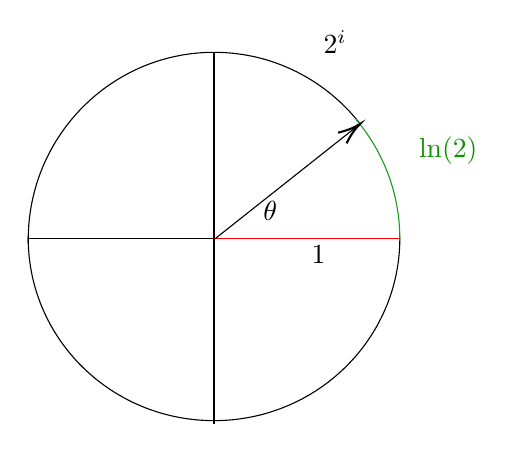
\begin{tikzpicture}[x=0.75pt,y=0.75pt,yscale=-1,xscale=1]
%uncomment if require: \path (0,300); %set diagram left start at 0, and has height of 300

%Straight Lines [id:da5300201460555855] 
\draw    (100,164.5) -- (189.5,164.5) ;
%Straight Lines [id:da7209499549539827] 
\draw    (189.5,254) -- (189.5,75) ;
%Shape: Arc [id:dp1477018513826992] 
\draw  [draw opacity=0] (100,167.2) .. controls (99.99,166.57) and (99.98,165.94) .. (99.98,165.31) .. controls (99.98,115.43) and (140.06,75) .. (189.51,75) .. controls (218.06,75) and (243.49,88.49) .. (259.88,109.49) -- (189.51,165.31) -- cycle ; \draw  [color={rgb, 255:red, 0; green, 0; blue, 0 }  ,draw opacity=1 ] (100,167.2) .. controls (99.99,166.57) and (99.98,165.94) .. (99.98,165.31) .. controls (99.98,115.43) and (140.06,75) .. (189.51,75) .. controls (218.06,75) and (243.49,88.49) .. (259.88,109.49) ;
%Straight Lines [id:da8647831039135583] 
\draw [color={rgb, 255:red, 255; green, 0; blue, 0 }  ,draw opacity=1 ]   (189.5,164.5) -- (279.02,164.5) ;
%Shape: Arc [id:dp5268217987140125] 
\draw  [draw opacity=0] (279.01,164.2) .. controls (279.01,164.3) and (279.02,164.4) .. (279.02,164.5) .. controls (279.02,213.08) and (238.94,252.46) .. (189.5,252.46) .. controls (140.06,252.46) and (99.98,213.08) .. (99.98,164.5) .. controls (99.98,164.29) and (99.99,164.08) .. (99.99,163.88) -- (189.5,164.5) -- cycle ; \draw   (279.01,164.2) .. controls (279.01,164.3) and (279.02,164.4) .. (279.02,164.5) .. controls (279.02,213.08) and (238.94,252.46) .. (189.5,252.46) .. controls (140.06,252.46) and (99.98,213.08) .. (99.98,164.5) .. controls (99.98,164.29) and (99.99,164.08) .. (99.99,163.88) ;
%Shape: Arc [id:dp1302089202448049] 
\draw  [draw opacity=0] (257.91,107.34) .. controls (271.09,122.89) and (279.03,143.02) .. (279.01,164.98) -- (189.91,164.9) -- cycle ; \draw  [color={rgb, 255:red, 22; green, 156; blue, 30 }  ,draw opacity=1 ] (257.91,107.34) .. controls (271.09,122.89) and (279.03,143.02) .. (279.01,164.98) ;
%Straight Lines [id:da04674799293912846] 
\draw    (189.91,164.9) -- (258.31,110.73) ;
\draw [shift={(259.88,109.49)}, rotate = 501.62] [color={rgb, 255:red, 0; green, 0; blue, 0 }  ][line width=0.75]    (10.93,-3.29) .. controls (6.95,-1.4) and (3.31,-0.3) .. (0,0) .. controls (3.31,0.3) and (6.95,1.4) .. (10.93,3.29)   ;

% Text Node
\draw (235.25,166.9) node [anchor=north west][inner sep=0.75pt]    {$1$};
% Text Node
\draw (287,114.4) node [anchor=north west][inner sep=0.75pt]  [color={rgb, 255:red, 12; green, 148; blue, 0 }  ,opacity=1 ]  {$\ln( 2)$};
% Text Node
\draw (241,63.4) node [anchor=north west][inner sep=0.75pt]    {$2^{i}$};
% Text Node
\draw (212,145.4) node [anchor=north west][inner sep=0.75pt]    {$\theta $};


\end{tikzpicture}

Note that we can represent any complex number in exponential form.
For example, \( (r, \theta) = re^{i \theta} \).

\begin{tikzpicture}[x=0.75pt,y=0.75pt,yscale=-1,xscale=1]
%uncomment if require: \path (0,300); %set diagram left start at 0, and has height of 300

%Curve Lines [id:da4423317108802115] 
\draw [color={rgb, 255:red, 255; green, 0; blue, 0 }  ,draw opacity=1 ]   (77.15,205.12) .. controls (201.44,203.62) and (289.8,139.23) .. (295.79,37.4) ;
%Straight Lines [id:da9534342452823479] 
\draw    (75.65,247.05) -- (297.28,247.05) ;
%Straight Lines [id:da33389606852560494] 
\draw    (75.65,35.9) -- (75.65,247.05) ;
%Shape: Circle [id:dp26393026690295507] 
\draw   (163,192) .. controls (163,190.9) and (163.9,190) .. (165,190) .. controls (166.1,190) and (167,190.9) .. (167,192) .. controls (167,193.1) and (166.1,194) .. (165,194) .. controls (163.9,194) and (163,193.1) .. (163,192) -- cycle ;
%Shape: Circle [id:dp10820914245059055] 
\draw   (123,201) .. controls (123,199.9) and (123.9,199) .. (125,199) .. controls (126.1,199) and (127,199.9) .. (127,201) .. controls (127,202.1) and (126.1,203) .. (125,203) .. controls (123.9,203) and (123,202.1) .. (123,201) -- cycle ;
%Shape: Circle [id:dp5803203757563192] 
\draw   (202,176) .. controls (202,174.9) and (202.9,174) .. (204,174) .. controls (205.1,174) and (206,174.9) .. (206,176) .. controls (206,177.1) and (205.1,178) .. (204,178) .. controls (202.9,178) and (202,177.1) .. (202,176) -- cycle ;
%Shape: Circle [id:dp5182181490141611] 
\draw   (255,137) .. controls (255,135.9) and (255.9,135) .. (257,135) .. controls (258.1,135) and (259,135.9) .. (259,137) .. controls (259,138.1) and (258.1,139) .. (257,139) .. controls (255.9,139) and (255,138.1) .. (255,137) -- cycle ;

% Text Node
\draw (71.9,262.4) node [anchor=north west][inner sep=0.75pt]    {$0$};
% Text Node
\draw (45,196.4) node [anchor=north west][inner sep=0.75pt]    {$1$};
% Text Node
\draw (167,193.4) node [anchor=north west][inner sep=0.75pt]  [color={rgb, 255:red, 255; green, 0; blue, 4 }  ,opacity=1 ]  {$e$};
% Text Node
\draw (163,263.4) node [anchor=north west][inner sep=0.75pt]    {$1$};
% Text Node
\draw (150,55.4) node [anchor=north west][inner sep=0.75pt]    {$e^{t}$};
% Text Node
\draw (127,202.4) node [anchor=north west][inner sep=0.75pt]    {$a$};
% Text Node
\draw (208,179.4) node [anchor=north west][inner sep=0.75pt]    {$b$};
% Text Node
\draw (261,140.4) node [anchor=north west][inner sep=0.75pt]    {$c$};


\end{tikzpicture}


\section{Identities}

We have \( \Re(z) = \frac{1}{2} (z + \bar z) \)
or \( \cos(x) = \frac{e^{ix} + e^{-ix}}{2} \).

\begin{tikzpicture}[x=0.75pt,y=0.75pt,yscale=-1,xscale=1]
%uncomment if require: \path (0,300); %set diagram left start at 0, and has height of 300

%Straight Lines [id:da34800919926202234] 
\draw [color={rgb, 255:red, 0; green, 0; blue, 0 }  ,draw opacity=1 ]   (99.75,227.18) -- (330.71,112.81) ;
\draw [shift={(332.5,111.93)}, rotate = 513.6600000000001] [color={rgb, 255:red, 0; green, 0; blue, 0 }  ,draw opacity=1 ][line width=0.75]    (10.93,-3.29) .. controls (6.95,-1.4) and (3.31,-0.3) .. (0,0) .. controls (3.31,0.3) and (6.95,1.4) .. (10.93,3.29)   ;
%Straight Lines [id:da63748929084913] 
\draw [color={rgb, 255:red, 255; green, 0; blue, 0 }  ,draw opacity=1 ]   (99.75,227.18) -- (219.09,168.63) ;
\draw [shift={(220.88,167.75)}, rotate = 513.87] [color={rgb, 255:red, 255; green, 0; blue, 0 }  ,draw opacity=1 ][line width=0.75]    (10.93,-3.29) .. controls (6.95,-1.4) and (3.31,-0.3) .. (0,0) .. controls (3.31,0.3) and (6.95,1.4) .. (10.93,3.29)   ;
%Straight Lines [id:da537720110515903] 
\draw [color={rgb, 255:red, 0; green, 95; blue, 255 }  ,draw opacity=1 ]   (220.88,167.75) -- (164.39,73.1) ;
\draw [shift={(163.36,71.38)}, rotate = 419.16999999999996] [color={rgb, 255:red, 0; green, 95; blue, 255 }  ,draw opacity=1 ][line width=0.75]    (10.93,-3.29) .. controls (6.95,-1.4) and (3.31,-0.3) .. (0,0) .. controls (3.31,0.3) and (6.95,1.4) .. (10.93,3.29)   ;
%Straight Lines [id:da16959396821644424] 
\draw    (99.75,227.18) -- (162.61,73.23) ;
\draw [shift={(163.36,71.38)}, rotate = 472.21] [color={rgb, 255:red, 0; green, 0; blue, 0 }  ][line width=0.75]    (10.93,-3.29) .. controls (6.95,-1.4) and (3.31,-0.3) .. (0,0) .. controls (3.31,0.3) and (6.95,1.4) .. (10.93,3.29)   ;
%Straight Lines [id:da8403058073952824] 
\draw    (99.75,227.18) -- (162.61,73.23) ;
\draw [shift={(163.36,71.38)}, rotate = 472.21] [color={rgb, 255:red, 0; green, 0; blue, 0 }  ][line width=0.75]    (10.93,-3.29) .. controls (6.95,-1.4) and (3.31,-0.3) .. (0,0) .. controls (3.31,0.3) and (6.95,1.4) .. (10.93,3.29)   ;

% Text Node
\draw (222.83,178.77) node [anchor=north west][inner sep=0.75pt]  [color={rgb, 255:red, 255; green, 0; blue, 0 }  ,opacity=1 ]  {$p=P_{u}( v)$};
% Text Node
\draw (202.31,100.35) node [anchor=north west][inner sep=0.75pt]  [color={rgb, 255:red, 0; green, 104; blue, 255 }  ,opacity=1 ]  {$v -p$};
% Text Node
\draw (149.98,43.4) node [anchor=north west][inner sep=0.75pt]    {$v$};
% Text Node
\draw (341.98,110.4) node [anchor=north west][inner sep=0.75pt]    {$u$};


\end{tikzpicture}


We have \( \Im(z) = \frac{1}{2}(z - \bar z) \)
or \( \sin(x) = \frac{e^{ix} - e^{-ix}}{2} \).

\begin{tikzpicture}[x=0.75pt,y=0.75pt,yscale=-1,xscale=1]
%uncomment if require: \path (0,300); %set diagram left start at 0, and has height of 300

%Shape: Axis 2D [id:dp6798239346637576] 
\draw  (82,202) -- (410.5,202)(140.5,8) -- (140.5,289) (403.5,197) -- (410.5,202) -- (403.5,207) (135.5,15) -- (140.5,8) -- (145.5,15) (173.5,197) -- (173.5,207)(206.5,197) -- (206.5,207)(239.5,197) -- (239.5,207)(272.5,197) -- (272.5,207)(305.5,197) -- (305.5,207)(338.5,197) -- (338.5,207)(371.5,197) -- (371.5,207)(107.5,197) -- (107.5,207)(135.5,169) -- (145.5,169)(135.5,136) -- (145.5,136)(135.5,103) -- (145.5,103)(135.5,70) -- (145.5,70)(135.5,37) -- (145.5,37)(135.5,235) -- (145.5,235)(135.5,268) -- (145.5,268) ;
\draw   ;
%Straight Lines [id:da44340582239633897] 
\draw    (139.5,200) -- (232.05,112.38) ;
\draw [shift={(233.5,111)}, rotate = 496.57] [color={rgb, 255:red, 0; green, 0; blue, 0 }  ][line width=0.75]    (10.93,-3.29) .. controls (6.95,-1.4) and (3.31,-0.3) .. (0,0) .. controls (3.31,0.3) and (6.95,1.4) .. (10.93,3.29)   ;
%Straight Lines [id:da7772236250141363] 
\draw  [dash pattern={on 0.84pt off 2.51pt}]  (233.5,111) -- (233.5,199) ;
%Straight Lines [id:da34998403337055295] 
\draw  [dash pattern={on 0.84pt off 2.51pt}]  (233.5,111) -- (142.95,25.37) ;
\draw [shift={(141.5,24)}, rotate = 403.4] [color={rgb, 255:red, 0; green, 0; blue, 0 }  ][line width=0.75]    (10.93,-3.29) .. controls (6.95,-1.4) and (3.31,-0.3) .. (0,0) .. controls (3.31,0.3) and (6.95,1.4) .. (10.93,3.29)   ;
%Straight Lines [id:da8180538641236395] 
\draw    (139.5,200) -- (233.02,284.66) ;
\draw [shift={(234.5,286)}, rotate = 222.15] [color={rgb, 255:red, 0; green, 0; blue, 0 }  ][line width=0.75]    (10.93,-3.29) .. controls (6.95,-1.4) and (3.31,-0.3) .. (0,0) .. controls (3.31,0.3) and (6.95,1.4) .. (10.93,3.29)   ;
%Straight Lines [id:da5851162400858174] 
\draw [color={rgb, 255:red, 255; green, 0; blue, 0 }  ,draw opacity=1 ]   (140.5,202) -- (141.49,26) ;
\draw [shift={(141.5,24)}, rotate = 450.32] [color={rgb, 255:red, 255; green, 0; blue, 0 }  ,draw opacity=1 ][line width=0.75]    (10.93,-3.29) .. controls (6.95,-1.4) and (3.31,-0.3) .. (0,0) .. controls (3.31,0.3) and (6.95,1.4) .. (10.93,3.29)   ;

% Text Node
\draw (226,88.4) node [anchor=north west][inner sep=0.75pt]    {$z$};
% Text Node
\draw (241,273.4) node [anchor=north west][inner sep=0.75pt]    {$\overline{z}$};
% Text Node
\draw (79,20.4) node [anchor=north west][inner sep=0.75pt]  [color={rgb, 255:red, 255; green, 0; blue, 0 }  ,opacity=1 ]  {$z-\overline{z}$};


\end{tikzpicture}

We have
\begin{align*}
    \cos(x + y) + i \sin(x + y) &= e^{i(x + y)} \\
    &= e^{ix} e^{iy} \\
    &= (C + i S)(c + i s) \\
    &= (Cc - Ss) + i (Sc + Cs)
\end{align*}
Thus
\[ \cos(x + y) = \cos(x) \cos(y) - \sin(x) \sin(y) \]
and
\[ \sin(x + y) = \sin(x) \cos(y) + \cos(x) \sin(y). \]


\tikzset{every picture/.style={line width=0.75pt}} %set default line width to 0.75pt

\noindent
\begin{tikzpicture}[x=0.75pt,y=0.75pt,yscale=-1,xscale=1]
%uncomment if require: \path (0,300); %set diagram left start at 0, and has height of 300

%Straight Lines [id:da3873432569541485] 
\draw    (52,149.5) -- (141.5,149.5) ;
%Straight Lines [id:da865029236905623] 
\draw    (141.5,239) -- (141.5,60) ;
%Shape: Arc [id:dp20510310643261065] 
\draw  [draw opacity=0] (52,152.2) .. controls (51.99,151.57) and (51.98,150.94) .. (51.98,150.31) .. controls (51.98,100.43) and (92.06,60) .. (141.51,60) .. controls (190.84,60) and (230.86,100.26) .. (231.03,149.99) -- (141.51,150.31) -- cycle ; \draw  [color={rgb, 255:red, 0; green, 0; blue, 0 }  ,draw opacity=1 ] (52,152.2) .. controls (51.99,151.57) and (51.98,150.94) .. (51.98,150.31) .. controls (51.98,100.43) and (92.06,60) .. (141.51,60) .. controls (190.84,60) and (230.86,100.26) .. (231.03,149.99) ;
%Straight Lines [id:da5752741725884877] 
\draw [color={rgb, 255:red, 255; green, 0; blue, 0 }  ,draw opacity=1 ]   (141.5,149.5) -- (231.02,149.5) ;
%Shape: Arc [id:dp9437146434068264] 
\draw  [draw opacity=0] (231.01,149.2) .. controls (231.01,149.3) and (231.02,149.4) .. (231.02,149.5) .. controls (231.02,198.08) and (190.94,237.46) .. (141.5,237.46) .. controls (92.06,237.46) and (51.98,198.08) .. (51.98,149.5) .. controls (51.98,149.29) and (51.99,149.08) .. (51.99,148.88) -- (141.5,149.5) -- cycle ; \draw   (231.01,149.2) .. controls (231.01,149.3) and (231.02,149.4) .. (231.02,149.5) .. controls (231.02,198.08) and (190.94,237.46) .. (141.5,237.46) .. controls (92.06,237.46) and (51.98,198.08) .. (51.98,149.5) .. controls (51.98,149.29) and (51.99,149.08) .. (51.99,148.88) ;
%Straight Lines [id:da4917580957488482] 
\draw    (141.51,150.31) -- (220.5,111) ;
%Straight Lines [id:da5810754421368048] 
\draw [color={rgb, 255:red, 0; green, 24; blue, 255 }  ,draw opacity=1 ]   (141.51,150.31) -- (200.5,84) ;
%Straight Lines [id:da7009838094462664] 
\draw  [dash pattern={on 0.84pt off 2.51pt}]  (220.5,111) -- (220.5,148) ;
%Straight Lines [id:da8582154760611198] 
\draw [color={rgb, 255:red, 0; green, 15; blue, 255 }  ,draw opacity=1 ] [dash pattern={on 0.84pt off 2.51pt}]  (200.5,84) -- (215.5,114) ;
%Shape: Right Triangle [id:dp02471566130097158] 
\draw   (509.71,84.06) -- (334,179) -- (520.93,144.02) -- cycle ;
%Shape: Right Triangle [id:dp13782255890731965] 
\draw   (543.5,142) -- (334,179) -- (543.5,179) -- cycle ;
%Shape: Arc [id:dp21455168656894863] 
\draw  [draw opacity=0] (421.54,47.99) .. controls (492.7,49.02) and (549.72,107.37) .. (549.03,178.61) .. controls (548.52,230.83) and (517.14,275.52) .. (472.4,295.52) -- (419.66,177.35) -- cycle ; \draw   (421.54,47.99) .. controls (492.7,49.02) and (549.72,107.37) .. (549.03,178.61) .. controls (548.52,230.83) and (517.14,275.52) .. (472.4,295.52) ;
%Straight Lines [id:da44468928407425945] 
\draw  [dash pattern={on 0.84pt off 2.51pt}]  (509.71,84.06) -- (509.71,180) ;
%Straight Lines [id:da7520054413333176] 
\draw    (251,174) -- (294.5,174) ;
\draw [shift={(296.5,174)}, rotate = 180] [color={rgb, 255:red, 0; green, 0; blue, 0 }  ][line width=0.75]    (10.93,-3.29) .. controls (6.95,-1.4) and (3.31,-0.3) .. (0,0) .. controls (3.31,0.3) and (6.95,1.4) .. (10.93,3.29)   ;
%Straight Lines [id:da13138036614687154] 
\draw [color={rgb, 255:red, 255; green, 0; blue, 0 }  ,draw opacity=1 ]   (520.93,83) -- (520.93,179) ;
%Straight Lines [id:da254833362509556] 
\draw [color={rgb, 255:red, 0; green, 6; blue, 255 }  ,draw opacity=1 ]   (509.71,84.06) -- (520.93,84.06) ;

% Text Node
\draw (187.25,151.9) node [anchor=north west][inner sep=0.75pt]    {$r$};
% Text Node
\draw (168,135.4) node [anchor=north west][inner sep=0.75pt]  [font=\footnotesize]  {$x$};
% Text Node
\draw (168,117.4) node [anchor=north west][inner sep=0.75pt]  [font=\footnotesize]  {$y$};
% Text Node
\draw (401,165.4) node [anchor=north west][inner sep=0.75pt]  [font=\footnotesize]  {$x$};
% Text Node
\draw (374,154.4) node [anchor=north west][inner sep=0.75pt]  [font=\footnotesize]  {$y$};
% Text Node
\draw (524,120.4) node [anchor=north west][inner sep=0.75pt]  [font=\footnotesize]  {$x$};


\end{tikzpicture}

See \( \cos(x) \cos(y) \) is shrinking \( \cos(x) \) up to the red,
and \( \sin(x) \sin(y) \) is taking the blue as a ratio to its hypotenuse.
And \( \sin(x) \cos(y) \) is shrinking \( \sin(x) \) up to red,
and \( \cos(x) \sin(y) \) is taking red of similar as ratio to its hypotenuse.

So \( \cos(2x) = \cos^2(x) - \sin^2(x) \)
and \( \sin(2x) = 2 \sin(x) \cos(x) \).



\end{document}
